\documentclass[12pt]{article}
\usepackage[utf8]{inputenc}
\usepackage[T1]{fontenc}
\usepackage[french]{babel}
\usepackage{amsmath, amssymb}
\usepackage{graphicx}
\usepackage{microtype}
\usepackage{tikz}
\usetikzlibrary{intersections, calc}
\usepackage{pgfplots}
\usepackage{hyperref}
\pgfplotsset{compat=newest}
\usepackage{listings}
\usepackage{xcolor}
\usepackage{amsthm}
\usepackage[margin=1in]{geometry}

\definecolor{codegreen}{rgb}{0,0.6,0}
\definecolor{codegray}{rgb}{0.5,0.5,0.5}
\definecolor{codepurple}{rgb}{0.58,0,0.82}
\definecolor{backcolour}{rgb}{0.95,0.95,0.92}
\usetikzlibrary{calc}

\lstdefinestyle{mystyle}{
    backgroundcolor=\color{backcolour},
    commentstyle=\color{codegreen},
    keywordstyle=\color{magenta},
    numberstyle=\tiny\color{codegray},
    stringstyle=\color{codepurple},
    basicstyle=\ttfamily\footnotesize,
    breakatwhitespace=false,
    breaklines=true,
    captionpos=b,
    keepspaces=true,
    numbers=left,
    numbersep=5pt,
    showspaces=false,
    showstringspaces=false,
    showtabs=false,
    tabsize=2
}

\lstset{style=mystyle}
\lstset{literate=%
{é}{{\'e}}{1}%
{è}{{\`e}}{1}%
{à}{{\`a}}{1}%
{ç}{{\c{c}}}{1}%
{œ}{{\oe}}{1}%
{ù}{{\`u}}{1}%
{É}{{\'E}}{1}%
{È}{{\`E}}{1}%
{À}{{\`A}}{1}%
{Ç}{{\c{C}}}{1}%
{Œ}{{\OE}}{1}%
{Ê}{{\^E}}{1}%
{ê}{{\^e}}{1}%
{î}{{\^i}}{1}%
{ô}{{\^o}}{1}%
{û}{{\^u}}{1}%
{ä}{{\"{a}}}1
{ë}{{\"{e}}}1
{ï}{{\"{i}}}1
{ö}{{\"{o}}}1
{ü}{{\"{u}}}1
{û}{{\^{u}}}1
{â}{{\^{a}}}1
{Â}{{\^{A}}}1
{Î}{{\^{I}}}1
}

\tolerance=2000
\emergencystretch=10pt
\newtheorem{lemma}{Lemme}
\newtheorem{remark}{Remarque}
\newtheorem{theorem}{Théorème}
\newtheorem{corollary}{Corollaire}
\newtheorem{definition}{Définition}
\newtheorem{proposition}{Proposition}
\newtheorem{example}{Exemple}

\title{Fonctions elliptiques de Weierstrass}
\author{}
\date{}

\begin{document}

\maketitle
\newpage
\tableofcontents
\newpage

\section*{Introduction}
Les fonctions elliptiques constituent un domaine fascinant et profondément riche de l'analyse complexe, ayant des applications étendues en théorie des nombres,
en physique et en ingénierie. Parmi ces fonctions, les fonctions elliptiques de Weierstrass jouent un rôle central grâce à leur structure élégante et leurs
propriétés intrinsèques. Ce travail a pour but de démystifier ces fonctions, en commençant par les fondements théoriques des fonctions holomorphes, méromorphes
et des singularités, et en avançant vers la définition précise et les applications des fonctions elliptiques de Weierstrass. En explorant ces concepts, nous
aborderons les aspects mathématiques et pratiques qui rendent les fonctions de Weierstrass non seulement intéressantes d'un point de vue théorique, mais également
précieuses pour diverses applications pratiques.

\newpage
\section{Rappels et Définitions}

\subsection{Fonction Holomorphe}
Soit $\Omega$ un domaine (ouvert non vide et connexe) de $\mathbb{C}$. Une fonction $f : \Omega \to \mathbb{C}$ est dite C-dérivable en $z_0 \in \Omega$ si la limite
\[
\lim_{z \to z_0} \frac{f(z) - f(z_0)}{z - z_0} = \lim_{h \to 0} \frac{f(z_0 + h) - f(z_0)}{h}
\]
existe dans $\mathbb{C}$. On la note alors $f'(z_0)$ et on l’appelle la dérivée de $f$ en $z_0$. La fonction $f$ est holomorphe sur $\Omega$ si elle est C-dérivable en tout point de $\Omega$. Dans ce cas, la fonction $z \mapsto f'(z)$, pour $z \in \Omega$, est appelée dérivée de $f$.

Une fonction entière est une fonction holomorphe sur l’ensemble $\mathbb{C}$ tout entier.

Une fonction $f$ est holomorphe en $z_0$ si elle est holomorphe sur un voisinage de $z_0$.\\

\textbf{Notation:} L’ensemble des fonctions holomorphes sur $\Omega$ sera noté $\Theta(\Omega)$.
\\ \\
\textit{Cette section est tirée du documents de cours Analyse Complexe du professeur Cyriaque ATINDOGBE, Mars 2022}
\subsection{Points Singuliers (Singularités)}
Soit $f : \mathbb{C} \to \mathbb{C}$. On dit que $z_0$ est une singularité de $f$ s'il existe un voisinage $V$ de $z_0$ tel que $f$ soit holomorphe en tout point de $V$ sauf en $z_0$.

La forme générale de la série de Laurent de $f$ sur une couronne $C(z_0, \tau_1, \tau_2)$, $0 \leq \tau_1 < \tau_2$, est donnée par :
\[
f(z) = \sum_{m=1}^{+\infty} a_{-m} (z - z_0)^{-m} + \sum_{n=0}^{+\infty} a_n (z - z_0)^n
\]
pour $z \in C(z_0, \tau_1, \tau_2)$.

On dit que $z_0$ est un pôle d'ordre $k$ de $f$ si pour tout $m > k$, $a_{-m} = 0$ et $a_{-k} \neq 0$.

\subsection{Fonction Méromorphe}
Une fonction $f$ est dite méromorphe sur le domaine $\Omega \subset \mathbb{C}$ si c'est une fonction $f : \Omega \to \mathbb{C}$ qui est holomorphe à l'exception de singularités isolées, toutes étant des pôles pour $f$.

Autrement dit, s'il existe un ensemble $A \subset \Omega$ tel que :
\begin{itemize}
    \item[(a)] $A$ n'a pas de point d'accumulation dans $\Omega$,
    \item[(b)] $f \in \Theta(\Omega \setminus A)$,
    \item[(c)] chaque point de $A$ est un pôle pour $f$.
\end{itemize}
L'ensemble des singularités de $f$ est appelé l'ensemble polaire de $f$.

\begin{remark}
\begin{itemize}
    \item Il est possible que $A = \emptyset$. Cela signifie que si nous notons $\mathcal{M}(\Omega)$ l'ensemble des fonctions méromorphes sur $\Omega$, on a : $\Theta(\Omega) \subset \mathcal{M}(\Omega)$.
    \item $A$ est au plus dénombrable puisque l'hypothèse (a) implique qu'aucune partie compacte de $\Omega$ ne contient une infinité de points de $A$.
\end{itemize}
\end{remark}

\textit{Cette section est tirée du documents de cours Analyse Complexe du professeur Cyriaque ATINDOGBE, Mars 2022}

\section*{Exemple 1 }
\section*{-La fonction}

\[ f(z) = \frac{g(z)}{(z - z_1)^{k_1} (z - z_2)^{k_2} \cdots (z - z_n)^{k_n}} \]
est méromorphe sur \( \mathbb{C} \). En effet:
\subsection*{}
1. \textbf{Fonction Holomorphe et Méromorphe}:
\begin{itemize}
	\item \( g(z) \) est holomorphe dans les voisinages de \( z_1, z_2, \ldots, z_n \) et est non nulle en chacun de ces points. Une fonction holomorphe est une fonction qui est différentiable en tout point de son domaine.
	\item Les fonctions \( (z - z_i)^{k_i} \) sont également holomorphes partout sauf en \( z_i \) où elles ont des pôles d'ordre \( k_i \).
	\item Une fonction est dite méromorphe si elle est holomorphe partout sauf en un ensemble de points isolés où elle peut avoir des pôles.
\end{itemize}

2. \textbf{Méromorphie de \( f(z) \)}:
\begin{itemize}
	\item Comme \( g(z) \) est holomorphe et non nulle aux voisinages des \( z_i \), \( g(z) \) n'introduit pas de nouvelles singularités en ces points.
	\item Les dénominateurs \( (z - z_i)^{k_i} \) introduisent des pôles en \( z_i \).
	\item Par conséquent, \( f(z) \) est holomorphe partout sauf aux points \( z_1, z_2, \ldots, z_n \) où elle a des pôles. Ceci implique que \( f(z) \) est méromorphe sur \( \mathbb{C} \).
\end{itemize}

\section*{-La fonction \(\tan(\pi z)\)}

\[ \tan(\pi z) = \frac{\sin(\pi z)}{\cos(\pi z)} \]
est méromorphe sur \( \mathbb{C} \). En effet:
\subsection*{}
1. \textbf{Pôles de \(\tan(\pi z)\)}:
\begin{itemize}
	\item La fonction \(\sin(\pi z)\) est holomorphe partout sur \( \mathbb{C} \).
	\item La fonction \(\cos(\pi z)\) est holomorphe partout sur \( \mathbb{C} \) et s'annule lorsque \(\pi z = \frac{\pi}{2} + k\pi\), c'est-à-dire lorsque \( z = \frac{1}{2} + k \) pour \( k \in \mathbb{Z} \).
\end{itemize}

2. \textbf{Singularités de \(\tan(\pi z)\)}:
\begin{itemize}
	\item Les zéros de \(\cos(\pi z)\) correspondent aux pôles de \(\tan(\pi z)\).
	\item À chaque point \( z = \frac{1}{2} + k \), \( \tan(\pi z) \) a un pôle simple car près de ces points, \(\cos(\pi z)\) se comporte comme une fonction linéaire (i.e., elle change de signe et sa dérivée est non nulle).
\end{itemize}

3. \textbf{Méromorphie de \(\tan(\pi z)\)}:
\begin{itemize}
	\item Hormis ces pôles simples, \(\tan(\pi z)\) est holomorphe partout ailleurs dans \( \mathbb{C} \).
	\item Par définition, une fonction qui est holomorphe partout sauf en un ensemble de pôles est méromorphe.
\end{itemize}

Ainsi, la fonction \(\tan(\pi z)\) est méromorphe sur \( \mathbb{C} \) avec des pôles simples en \( z = \frac{1}{2} + k \), \( k \in \mathbb{Z} \).


\subsection{Réseau de $\mathbb{C}$}
Un sous-groupe additif $\Lambda \subset \mathbb{C}$ est un réseau si :
\begin{enumerate}
    \item $\Lambda$ est discret,
    \item $\Lambda$ engendre $\mathbb{C}$ sur $\mathbb{R}$.
\end{enumerate}

\textit{Cette définition est extraite du travail d'étude de recherche réaliser par ARGOUD Thomas sur les fonctions elliptiques.}
\section*{Exemple 2 : Le réseau généré par \(1\) et \(i\)}

Considérons le sous-groupe \(\Lambda\) de \(\mathbb{C}\) engendré par les éléments \(1\) et \(i\) (l'unité imaginaire) :
\[
\Lambda = \{ m + ni \mid m, n \in \mathbb{Z} \}
\]

\textbf{Discret :} Les points de \(\Lambda\) sont de la forme \(m + ni\), où \(m\) et \(n\) sont des entiers. Il n'y a donc pas de points de \(\Lambda\) arbitrairement proches les uns des autres ; en effet, la distance minimale entre deux points distincts de \(\Lambda\) est au moins \(1\) (car les plus proches voisins sont distants de 1).

\textbf{Engendre \(\mathbb{C}\) sur \(\mathbb{R}\) :} Tout nombre complexe \(z \in \mathbb{C}\) peut s'écrire comme \(a + bi\), où \(a\) et \(b\) sont des réels. Comme \(\Lambda\) contient \(1\) et \(i\), il est possible de générer tout complexe \(a + bi\) en combinant \(1\) et \(i\) avec des coefficients réels.

Ainsi, \(\Lambda = \{ m + ni \mid m, n \in \mathbb{Z} \}\) est un réseau.

\section*{Exemple 3 : Le réseau généré par \(1\) et \(\omega\), où \(\omega = e^{2\pi i / 3}\)}

Prenons le sous-groupe \(\Lambda\) de \(\mathbb{C}\) engendré par \(1\) et \(\omega\), où \(\omega = e^{2\pi i / 3} = -\frac{1}{2} + i\frac{\sqrt{3}}{2}\) (une racine cubique primitive de l'unité) :
\[
\Lambda = \{ m + n\omega \mid m, n \in \mathbb{Z} \}
\]

\textbf{Discret :} Les points de \(\Lambda\) sont de la forme \(m + n\omega\). Comme \(\omega\) est un nombre complexe non réel, les points de \(\Lambda\) sont espacés et ne peuvent pas être arbitrairement proches les uns des autres.

\textbf{Engendre \(\mathbb{C}\) sur \(\mathbb{R}\) :} Tout nombre complexe \(z \in \mathbb{C}\) peut s'écrire comme une combinaison linéaire de \(1\) et \(\omega\) avec des coefficients réels. En effet, \(1\) et \(\omega\) sont linéairement indépendants sur \(\mathbb{R}\) et forment une base pour \(\mathbb{C}\) en tant qu'espace vectoriel réel.

Donc, \(\Lambda = \{ m + n\omega \mid m, n \in \mathbb{Z} \}\) est également un réseau.

Ces deux exemples illustrent bien la structure d'un réseau dans \(\mathbb{C}\) en satisfaisant les deux conditions requises.
\subsection{Périodicités de fonctions Méromorphes}
\begin{definition}	
 \quad Une fonction méromorphe \( f: \mathbb{C} \to \mathbb{C} \) est dite \textit{périodique de période} \( \tau \in \mathbb{C}^* \) si pour tout \( z \) dans \( \mathbb{C} \):
\[ 
z + \tau \in \Omega \quad \text{et} \quad f(z + \tau) = f(z) 
\]
\textit{Cette définition est extraite du travail d'étude de recherche réaliser par ARGOUD Thomas sur les fonctions elliptiques.}
\end{definition}
\section*{Exemple 4 : }

La fonction exponentielle \( f(z) = e^z \) est une fonction méromorphe et elle est périodique de période \( 2\pi i \). En effet, pour tout \( z \in \mathbb{C} \) :

\[
f(z + 2\pi i) = e^{z + 2\pi i} = e^z \cdot e^{2\pi i} = e^z \cdot 1 = e^z = f(z)
\]

Ainsi, \( e^z \) est une fonction méromorphe périodique de période \( 2\pi i \).

\begin{remark}
 Il n'y a pas unicité de la période d'une telle fonction, en effet, pour tout \( \lambda \) dans \( \tau \mathbb{Z} \), \( \lambda\) est une période de \( f \).
 \end{remark}
On note \( \Lambda_f \) l'ensemble des périodes de la fonction \( f \).

\begin{proposition}
Soit \( f \) une fonction méromorphe non constante, de trois choses l'une:

    
 
\begin{enumerate}
    \item \( \Lambda_f = \emptyset \)
    \item Il existe \( \tau_1 \in \mathbb{C}^* \) une période de \( f \) avec \( |\tau_1| \) minimal tel que \( \Lambda_f = \tau_1 \mathbb{Z}^* \)
    \item Il existe \( \tau_1, \tau_2 \in \mathbb{C}^* \) deux périodes de \( f \) telles que:
    \[
    \frac{\tau_1}{\tau_2} \notin \mathbb{R} \quad \text{et} \quad \forall \tau \in \Lambda_f:  \exists! (n, m) \in \mathbb{Z}^2, \quad \tau = n\tau_1 + m\tau_2
    \]
\end{enumerate}
\end{proposition}
Nous appellerons de telles périodes \( \tau_1 \) et \( \tau_2 \) des périodes fondamentales de \( f \).
	
\section*{Exemple 5}
	Pour chaque situation décrite, nous pouvons proposer des exemples spécifiques de fonctions méromorphes non constantes.

\textbf{Cas 1 :} \(\Lambda_f = \emptyset\)

Cela signifie que la fonction \( f \) n'a pas de périodes. Un exemple de telle fonction est la fonction rationnelle \(\frac{1}{z}\), qui est méromorphe mais n'a pas de période. Autrement dit, pour tout \(\tau \in \mathbb{C}^*\), \(\frac{1}{z + \tau} \neq \frac{1}{z}\).

\textbf{Cas 2 :} \(\Lambda_f = \tau_1 \mathbb{Z}\)

Cela signifie que la fonction \( f \) a une période \(\tau_1\) avec \(|\tau_1|\) minimal, et \(\Lambda_f\) est généré par cette seule période. Un exemple de telle fonction est la fonction exponentielle \( e^z \), qui a une période \(2\pi i\) :
\[
f(z + 2\pi i) = e^{z + 2\pi i} = e^z \cdot e^{2\pi i} = e^z
\]
Ainsi, \(\tau_1 = 2\pi i\) et \(\Lambda_f = 2\pi i \mathbb{Z}\).

\textbf{Cas 3 :} \(\Lambda_f\) est engendré par deux périodes fondamentales \(\tau_1\) et \(\tau_2\)

Cela signifie que la fonction \( f \) a deux périodes \(\tau_1\) et \(\tau_2\) telles que \(\frac{\tau_1}{\tau_2} \notin \mathbb{R}\) et que chaque période de \( f \) est une combinaison linéaire entière de \(\tau_1\) et \(\tau_2\). Un exemple classique de telle fonction est la fonction de Weierstrass \(\wp(z)\), qui est doublement périodique :
\[
\wp(z + \omega_1) = \wp(z) \quad \text{et} \quad \wp(z + \omega_2) = \wp(z)
\]
où \(\omega_1\) et \(\omega_2\) sont les périodes fondamentales du réseau \(\Lambda\), avec \(\frac{\omega_1}{\omega_2} \notin \mathbb{R}\).

Un autre exemple est la fonction cotangente elliptique \(\cot(\pi z)\), qui est aussi doublement périodique avec les périodes \(1\) et \(i\) :
\[
\cot(\pi (z + 1)) = \cot(\pi z) \quad \text{et} \quad \cot(\pi (z + i)) = \cot(\pi z)
\]
Dans ces deux exemples, les périodes fondamentales \(\tau_1\) et \(\tau_2\) ne sont pas colinéaires sur \(\mathbb{R}\), satisfaisant ainsi les conditions pour le cas 3.

En résumé :

\begin{itemize}
	\item Exemple pour \(\Lambda_f = \emptyset\) : \(\frac{1}{z}\)
	\item Exemple pour \(\Lambda_f = \tau_1 \mathbb{Z}\) : \(e^z\) avec \(\tau_1 = 2\pi i\)
	\item Exemple pour \(\Lambda_f\) avec deux périodes fondamentales : \(\wp(z)\) (périodes \(\omega_1\) et \(\omega_2\)) et \(\cot(\pi z)\) (périodes \(1\) et \(i\))
\end{itemize}

\vspace{0.5cm}
Pour démontrer cette proposition, nous allons énoncer la proposition et le lemme suivant.

\begin{proposition} \quad Toute fonction méromorphe avec trois périodes indépendantes est constante. \end{proposition}

\begin{remark}
\begin{itemize}
    \item[(i)] Le théorème nous dit en réalité que si nous sommes dans le 3\textsuperscript{ème} cas: \( \Lambda_f = \tau_1 \mathbb{Z} + \tau_2 \mathbb{Z} \); \( \tau_1 \) et \( \tau_2 \) sont des périodes fondamentales de \( f \).
    \item[(ii)] Il n'y a pas unicité des périodes fondamentales de \( f \), par exemple, \( \pm \tau_1 \) et \( \pm \tau_2 \) sont aussi des périodes fondamentales.
    \item[(iii)] Toute fonction vérifiant le 3\textsuperscript{ème} cas est dite doublement périodique.
\end{itemize}

\begin{figure}[h]
    \centering
    \begin{tikzpicture}[scale=1.5]
        % Define the grid
        \foreach \x in {0,1,2,3,4,5}
        \foreach \y in {0,1,2,3}
        {
            \draw (\x,\y) -- (\x+1,\y); % horizontal lines
            \draw (\x,\y) -- (\x,\y+1); % vertical lines
        }
        
        % Add the last set of lines to complete the grid
        \foreach \y in {0,1,2,3}
        {
            \draw (6,\y) -- (6,\y+1);
        }
        \foreach \x in {0,1,2,3,4,5,6}
        {
            \draw (\x,4) -- (\x+1,4);
        }
        
        % Labels and specific vectors
        \draw[thick, red, ->] (3,2) -- node[below] {$\tau_1$} (4,2);
        \draw[thick, red, ->] (3,2) -- node[left] {$\tau_2$} (3,3);
    \end{tikzpicture}
    \caption{Illustration du 3\textsuperscript{ème} cas}
\end{figure}
\end{remark}
\begin{lemma}
Soit \( f \) une fonction périodique non constante, l'ensemble \( \Lambda_f \) ne contient pas de point d'accumulation, c'est un ensemble discret de \( \mathbb{C} \).
\end{lemma}

\begin{proof}[\textbf{Démonstration (Lemme 1)}]
On démontre ce lemme par l'absurde. Posons \( \alpha \in \Lambda_f \) un point d'accumulation et soit \( P \) l'ensemble des pôles de \( f \). Il existe une suite \( (\tau_n) \) de \( \Lambda_f \) telle que \( (\tau_n) \) converge vers \( \alpha \) et pour tout \( i \neq j \), \( \tau_i \neq \tau_j \). Soit \( z_0 \in \mathbb{C}\setminus P \), \( z_0 + \alpha \in \mathbb{C}\setminus P \) car \( \alpha \in \Lambda_f \), par continuité de la fonction \( f \) et périodicité : 
\[
f(z_0 + \alpha) = \lim_{n \to \infty} f(z_0 + \tau_n) = f(z_0)
\]
Ainsi, \( z_0 + \alpha \) est un zéro non isolé de la fonction méromorphe \( f - f(z_0) \). Par le théorème des zéros isolés, \( f - f(z_0) \) est identiquement nulle, donc \( f \equiv f(z_0) \), ce qui est impossible car \( f \) est supposée non constante.
\end{proof}
\begin{remark}
    Pour tout \( A \) non vide tel que \( A \subseteq \Lambda_f \), il existe \( \tilde{r} \in A \) tel que :
    \[ 
    |\tilde{r}| = \inf\{|r| : r \in A\} 
    \]
    En effet, $ \{|r| : r \in A\} $ est une partie non vide minorée par 0 sans point d'accumulation. Elle admet donc un minimum.
\end{remark}

\begin{proof}[\textbf{Démonstration de la proposition 1.}] \

Si \( \Lambda_f = \{0\} \), nous sommes dans le 1\textsuperscript{er} cas. On suppose donc maintenant que \( \Lambda_f \neq \{0\} \).

D'après la remarque précédente, on sait qu'il existe \( \tau_1 \in \Lambda_f \) tel que
\[
|\tau_1| = \inf\{|r| : r \in \Lambda_f\}
\]
Posons \( B = \tau_1\mathbb{Z} \). Il est immédiat que \( B \subseteq \Lambda_f \).

Si \( B = \Lambda_f \), nous sommes dans le 2\textsuperscript{ème} cas, en revanche si \( B \neq \Lambda_f \), il faut montrer que nous sommes dans le 3\textsuperscript{ème} cas.

Si \( B = \Lambda_f \), nous sommes dans le 2\textsuperscript{ème} cas, en revanche si \( B \neq \Lambda_f \), il faut montrer que nous sommes dans le 3\textsuperscript{ème} cas.

En utilisant à nouveau la remarque pour \( \Lambda_f \setminus B  \), il existe \( \tau_2 \in \Lambda_f \setminus B  \) tel que
\[
|\tau_2| = \inf\{|r| : r \in \Lambda_f \setminus B \}
\]

Alors \( \lambda \in \mathbb{R}\setminus\mathbb{Z} \), car \( \tau_2 \in \Lambda_f \setminus B  \), et de plus \( \tau_2 - \lambda\tau_1 = (\lambda - 1)\tau_1 \in \Lambda_f \), avec \( \lambda - 1 \neq 0 \); ce qui est impossible d'après la définition de \( \tau_1 \).
\begin{itemize}
    \item Montrons pour commencer que \( \frac{\tau_1}{\tau_2} \notin \mathbb{R} \). Supposons par l'absurde qu'il existe \( \lambda \in \mathbb{R} \) tel que \( \tau_2 = \lambda\tau_1 \).
    Alors \( \lambda \in \mathbb{R} \setminus \mathbb{Z} \), car \( \tau_2 \in \Lambda_f \setminus B \) et de plus  \[
    \tau_2 - \lfloor \lambda \rfloor \tau_1 = (\lambda - \lfloor \lambda \rfloor) \tau_1 \in \Lambda_f, \quad \text{avec} \quad \lambda - \lfloor \lambda \rfloor \in ]0, 1[
        \], ce qui est impossible d’après la définition de \( \tau_1 \).
    \item Montrons maintenant que toute période \( \tau \) de \( \Lambda_f \) peut s'écrire de manière unique sous la forme
    \[
        \tau = n\tau_1 + m\tau_2, \quad n, m \in \mathbb{Z}.
        \]
    \end{itemize}

    En effet, puisque \(\frac{\tau_1}{\tau_2} \notin \mathbb{R}\), \((\tau_1, \tau_2)\) forme une base de \(\mathbb{C}\) en tant que \(\mathbb{R}\) espace vectoriel; ce qui entraîne l’existence de deux scalaires uniques \(\lambda_1\) et \(\lambda_2\) tels que \(\tau = \lambda_1 \tau_1 + \lambda_2 \tau_2\). De plus, il existe deux entiers \(n_1\) et \(n_2\) tels que \(|\lambda_1 - n_1| \leq \frac{1}{2}\) et \(|\lambda_2 - n_2| \leq \frac{1}{2}\).
    
    Ainsi :
    
    \((\lambda_1 - n_1)\tau_1 + (\lambda_2 - n_2)\tau_2 = \tau - n_1\tau_1 - n_2\tau_2 \in \Lambda_f\)
    
    
    Par conséquent:
    \begin{enumerate}
    \item Si \(\lambda_1 - n_1 = \lambda_2 - n_2 = 0\), alors \(\tau = n_1\tau_1 + n_2\tau_2\).
    \item Si \(\lambda_1 - n_1 = 0\) et \(\lambda_2 - n_2 \neq 0\), alors \((\lambda_2 - n_2)\tau_2 \in \Lambda_f\) et \(\left|(\lambda_2 - n_2)\tau_2\right| \leq |\tau_2|\).\
    Donc, par définition de \(\tau_2\), \((\lambda_2 - n_2)\tau_2 \in B\), d’où l’existence d’un \(n \in \mathbb{Z}\) tel que \(\tau = n_1\tau_1 + n_2\tau_2\).
    \item Le cas \(\lambda_1 - n_1 \neq 0\) et \(\lambda_2 - n_2 = 0\) est impossible car \((\lambda_1 - n_1)\tau_1\ \in \Lambda_f\) et \(\left|(\lambda_1 - n_1)\tau_1\right| < |\tau_1|\), ce qui contredit la définition de \(\tau_1\).
    \item Si \((\lambda_1 - n_1)(\lambda_2 - n_2) \neq 0\), on a, puisque \(\frac{\tau_1}{\tau_2} \notin \mathbb{R}\):
    
    \(\left|\tau - n_1\tau_1 - n_2\tau_2\right| \leq \left|(\lambda_1 - n_1)\tau_1\right| + \left|(\lambda_2 - n_2)\tau_2\right| \leq \frac{1}{2}\left(|\tau_1| + |\tau_2|\right) \leq |\tau_2|\)
    
    Donc, par définition de \(\tau_2\), \((\tau -n_1\tau_1 - n_2\tau_2 \in B)\), d’où l’existence d’un \(n \in \mathbb{Z}\) tel que \(\tau = n_1\tau_1 + n_2\tau_2\).
    \end{enumerate}

\end{proof}



    \section{Fonctions élliptiques}
    \textit{Ce  chapitre est inspiré du travail d'étude de recherche réaliser par ARGOUD Thomas  sur les fonctions elliptiques.}

    Dans cette section, nous allons nous intéresser aux résultats principaux des fonctions elliptiques avant d’expliciter des exemples dans la section suivante.
    \subsection{Définitions }
    \begin{definition}(Fonction elliptique)
    
    On appelle \textit{fonction elliptique} toute fonction méromorphe dans $\mathbb{C}$ non constante et doublement périodique.
    \end{definition}
    \begin{definition}(Parallélogramme)
    
    Soient $a \in \mathbb{C}$ et $\omega_1, \omega_2 \in \mathbb{C}^{*}$, on appelle \textit{parallélogramme} dans $\mathbb{C}$ l’ensemble :
    
    \[
\mathcal{P}_{a}{(\omega_1, \omega_2)} = \{ a + \alpha \omega_1 + \beta \omega_2 \mid 0 \leq \alpha, \beta < 1 \}
\]
\end{definition}
    
    Dans le cas où $f$ est une fonction elliptique de périodes fondamentales $\omega_1$ et $\omega_2$ et $a = 0$, on parlera d’un \textit{parallélogramme fondamental} de $f$. On le notera dans la suite $\mathcal{P}{(\omega_1, \omega_2)}$.
    
    \begin{center}
        \begin{figure}[h]
            \centering
            \begin{tikzpicture}
            \coordinate (O) at (0,0);
            \coordinate (A) at (2,0);
            \coordinate (B) at (1,2);
            \coordinate (C) at ($(A) + (B)$);
            \draw[thick] (O) -- (A) -- (C) -- (B) -- cycle;
            \draw[dashed] (O) -- (B);
            \draw[dashed] (A) -- (C);
        
            \node at (-0.2,-0.2) {$a$};
            \node at (2.2,-0.2) {$a + \omega_1$};
            \node at (1,2.2) {$a + \omega_2$};
            \node at (3.2,2.2) {$a + \omega_1 + \omega_2$};
            \end{tikzpicture}
            \caption{Illustration d’un parallélogramme issu de $a$.}
        \end{figure}
\end{center}

\newpage
 
 	\section*{\textbf{Exemple 6 :} La fonction \(\wp\) de Weierstrass}
 
 La fonction de Weierstrass \(\wp(z)\) est une fonction elliptique doublement périodique avec des périodes fondamentales \(\omega_1\) et \(\omega_2\). Le parallélogramme fondamental \(P(\omega_1, \omega_2)\) pour cette fonction est défini par :
 \[ P(\omega_1, \omega_2) = \left\{ \alpha \omega_1 + \beta \omega_2 \mid 0 \leq \alpha, \beta < 1 \right\} \]
 
 Exemple concret : Prenons \(\omega_1 = 1\) et \(\omega_2 = i\). Alors le parallélogramme fondamental \(P(1, i)\) pour la fonction \(\wp(z)\) est :
 \[ P(1, i) = \left\{ \alpha + \beta i \mid 0 \leq \alpha, \beta < 1 \right\} \]
 Cela représente le carré dans le plan complexe avec les sommets \(0\), \(1\), \(i\), et \(1 + i\).
 
 \section*{\textbf{Exemple 7 :} La fonction \(\sigma\) de Weierstrass}
 
 La fonction \(\sigma(z)\) de Weierstrass est une autre fonction elliptique liée à \(\wp(z)\) et elle a les mêmes périodes fondamentales \(\omega_1\) et \(\omega_2\). Le parallélogramme fondamental \(P(\omega_1, \omega_2)\) pour cette fonction est également défini de la même manière :
 \[ P(\omega_1, \omega_2) = \left\{ \alpha \omega_1 + \beta \omega_2 \mid 0 \leq \alpha, \beta < 1 \right\} \]
 
 Exemple concret : Prenons \(\omega_1 = 2\pi\) et \(\omega_2 = 2\pi i\). Alors le parallélogramme fondamental \(P(2\pi, 2\pi i)\) pour la fonction \(\sigma(z)\) est :
 \[ P(2\pi, 2\pi i) = \left\{ 2\pi \alpha + 2\pi i \beta \mid 0 \leq \alpha, \beta < 1 \right\} \]
 Cela représente un rectangle dans le plan complexe avec les sommets \(0\), \(2\pi\), \(2\pi i\), et \(2\pi + 2\pi i\).
 
 Ces deux exemples montrent comment les périodes fondamentales \(\omega_1\) et \(\omega_2\) définissent un parallélogramme fondamental pour les fonctions elliptiques \(\wp(z)\) et \(\sigma(z)\), qui sont toutes deux doublement périodiques.
\subsection{Théorème de Liouville}
\begin{theorem}(Théorème de Liouville)

Toute fonction elliptique holomorphe sur $\mathbb{C}$ est constante.
\end{theorem}
Pour la démonstration de ce théorème, nous allons énoncer et démontrer le lemme suivant.
\begin{lemma}
    Soient $a \in \mathbb{C}$ et $\omega_1, \omega_2 \in \mathbb{C}^{*}$ tels que $\frac{\omega_1}{\omega_2} \notin \mathbb{R}$. Alors pour tout $z$ dans $\mathbb{C}$, on peut associer un unique $z’ \in \mathcal{P}_{a}{(\omega_1, \omega_2)}$ et deux uniques $n, m \in \mathbb{Z}$ tels que $z = z’ + n \omega_1 + m \omega_2$.
\end{lemma}
\begin{proof}[\textbf{Démonstration du Lemme}] \
La démonstration est similaire à celle du précédent lemme en considérant $z-a$.
En effet, $\frac{\omega_1}{\omega_2} \notin \mathbb{R}$ donc $\{ \omega_1, \omega_2 \}$ est une base de $\mathbb{C}$ en tant que $\mathbb{R}$ espace vectoriel, ce qui entraîne l'existence de deux scalaires uniques $\alpha, \beta \in \mathbb{R}$ tels que :
\[
z - a = \alpha \omega_1 + \beta \omega_2 = (\alpha - \lfloor \alpha \rfloor) \omega_1 + (\beta - \lfloor \beta \rfloor) \omega_2 + \lfloor \alpha \rfloor \omega_1 + \lfloor \beta \rfloor \omega_2
\]
\[
    (\alpha - \lfloor \alpha \rfloor), (\beta - \lfloor \beta \rfloor)  \in ]0, 1[
\]

Donc on a bien montré l'existence d'une telle décomposition, il faut désormais montrer l'unicité. Pour cela, supposons que :
\[
z_1 + n_1 \omega_1 + m_1 \omega_2 = z = z_2 + n_2 \omega_1 + m_2 \omega_2
\]
et donc
\[
z_1 - z_2 = (n_2 - n_1) \omega_1 + (m_2 - m_1) \omega_2
\]
De plus, $z_1, z_2 \in \mathcal{P}_{a}(\omega_1, \omega_2)$, donc il existe $r, s \in  ]-1, 1[$ tels que $z_2 - z_1 = r \omega_1 + s \omega_2$

Par unicité de la décomposition dans la base ${\left\{ \omega_1, \omega_2\right\}}$ on en déduit :
\[
\begin{cases}
r = n_1 - n_2 \in \mathbb{Z} \\
s = m_1 - m_2 \in \mathbb{Z}
\end{cases}
\implies
\begin{cases}
r = 0 \\
s = 0
\end{cases}
\quad \text{car le seul entier entre -1 et 1 est 0}
\]

D'où l'unicité.
\end{proof}
\begin{remark}
    Grâce à ce lemme, nous pouvons en déduire l’égalité suivante :
\[
\mathbb{C} = \bigcup_{\gamma \in \Lambda_{f}} \mathcal{P}_{\alpha + \gamma} (\omega_1, \omega_2)
\]

\begin{figure}[h]
\centering
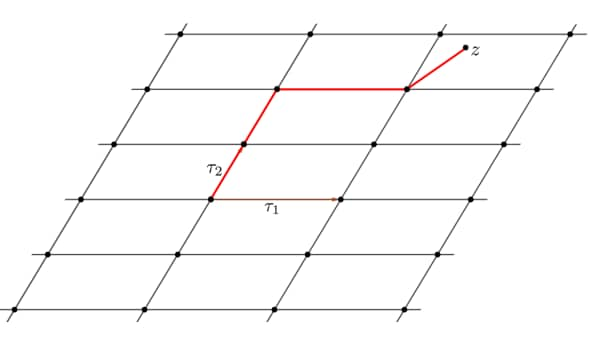
\includegraphics[width=0.6\textwidth]{lemme.jpeg}
\caption{Illustration du \textit{lemme} 2 et de l’\textit{égalité} précédente}
\end{figure}
\end{remark}

\begin{proof}[\textbf{Démonstration du Théorème de Liouville}]
Soit $\mathcal{P}(\omega_1, \omega_2)$ un parallélogramme fondamental de $f$.

La fonction $f$ étant holomorphe sur $\mathbb{C}$, elle est donc continue et ainsi bornée sur $\partial \mathcal{P}(\omega_1, \omega_2)$, et par le principe du maximum, $f$ est bornée sur $\mathcal{P}(\omega_1, \omega_2)$.

Ainsi, d’après le lemme 2, tout nombre complexe $z$ peut s’écrire sous la forme :

\[ z = z’ + n \omega_1 + m \omega_2 \quad \text{avec} \quad z’ \in \mathcal{P}(\omega_1, \omega_2), \quad n, m \in \mathbb{Z} \]

On en déduit donc :

\[ \sup_{z \in \mathbb{C}} |f(z)| = \sup_{z’ \in \mathcal{P}(\omega_1, \omega_2)} |f(z’)| < +\infty \]

La fonction $f$ est donc bornée et entière, donc constante par le théorème de Liouville.
\end{proof}

\subsection{Ordre d’une fonction elliptique}

Soit $z \in \mathbb{C}$. D’après le lemme 2, il existe $\zeta \in \mathcal{P}(\omega_1, \omega_2)$ et $n, m \in \mathbb{Z}$ tels que $z = \zeta + n \omega_1 + m \omega_2$. Vient alors :

\begin{proposition}
    $z \in \mathbb{C}$ est un zéro ou un pôle d’ordre $p$ d’une fonction elliptique $f$ si et seulement si $\zeta$ est respectivement un zéro ou un pôle d’ordre $p$.

\end{proposition}

\begin{proof}[\textbf{Démonstration de la proposition}]

Si $z$ est un pôle d'ordre $p$, par la caractérisation des pôles il existe $c$ tel que l'on ait :
\[
\lim_{h \to 0} h^p f(z + h) = c \iff \lim_{h \to 0} h^p f(\zeta + n\omega_1 + m\omega_2 + h) = c
\]
\[
\iff \lim_{h \to 0} h^p f(\zeta + h) = c
\]
\[
\iff \zeta \text{ est un pôle d'ordre } p \text{ de } f
\]

Si $z$ est un zéro d'ordre $p$. Remarquons que si $f$ est elliptique, $\frac{1}{f}$ est aussi elliptique ($\mathbb{C}$ est connexe donc $\mathcal{M}(\mathbb{C})$ est un corps, $\frac{1}{f}$ est donc méromorphe), ainsi on a :

$z$ est un zéro d'ordre $p$ de $f \iff z $ est un pôle d'ordre $p$ de $\frac{1}{f}$ 
\[
\iff \zeta \text{ est un pôle d'ordre } p \text{ de } \frac{1}{f}
\]
\[
\iff \zeta \text{ est un zéro d'ordre } p \text{ de } f
\]

Ce qui complète la démonstration de la proposition.
\end{proof}

\begin{theorem} \
Toute fonction elliptique $f$ possède au moins un pôle dans $\mathcal{P}(\omega_1, \omega_2)$.
\end{theorem}
\begin{proof}[\textbf{Démonstration}]

Par l’absurde, supposons que $f$ ne possède aucun pôle dans $\mathcal{P}(\omega_1, \omega_2)$. Par la proposition 3, $f$ ne possède alors aucun pôle dans $\mathbb{C}$, ce qui implique que $f$ est entière. En conséquence, $f$ est une constante, ce qui est une contradiction.
\end{proof}
\begin{proposition} \
Le nombre fini de pôles (compté avec multiplicité) d’une fonction elliptique $f$ dans un de ses parallélogrammes fondamentaux $\mathcal{P}(\omega_1, \omega_2)$ est appelé l’ordre de $f$.
\end{proposition}
\begin{proof}[\textbf{Démonstration}]

Pour que cette définition ait un sens, il faut montrer que le nombre de pôles (compté avec multiplicité) est indépendant de la paire de périodes fondamentales.

Soient $(\omega_1, \omega_2)$ et $(\omega’_1, \omega’_2)$ deux paires de périodes fondamentales de $f$. Désignons par $A$ et $B$ respectivement les pôles de $f$ dans $\mathcal{P}(\omega_1, \omega_2)$ et $\mathcal{P}(\omega’_1, \omega’_2)$.

D’après le théorème 2 et le lemme 2, $A$ et $B$ sont non vides et finis. Définissons une fonction :
\[
j: A \rightarrow B
\]
\[
z \mapsto \zeta  
\]
\[
    \text{avec} \quad z \mapsto \zeta + n\omega'_1 + m\omega'_2, \quad \zeta \in B \quad \text{et} \quad n,m \in \mathbb{Z}.
    \] 
Cette fonction est bien définie par unicité de la décomposition de $z$ démontrée dans le lemme 2. Il suffit alors de montrer que $j$ est bijective pour obtenir le résultat voulu.

Soit $z_1, z_2 \in A$ tels que $j(z_1) = j(z_2)$. Alors, $z_1 - z_2 \in \Lambda_f$ et il existe, puisque $(\omega_1, \omega_2)$ est une paire de périodes fondamentales et de ce fait forme une base de $\mathbb{C}$ en tant que $\mathbb{R}$-espace vectoriel, deux scalaires $r$ et $s$ tels que :

\[ z_1 - z_2 = r\omega_1 + s\omega_2 \]

De plus, comme $z_1, z_2 \in \mathcal{P}(\omega_1, \omega_2)$ et $z_1 - z_2 \in \Lambda_f$, on a $-1 < r, s < 1$ avec $r, s \in \mathbb{Z}$.

Par conséquent, par l’unicité d’une telle décomposition, $r = s = 0$ et on a bien $z_1 = z_2$.

Soit $c \in B$. Alors, il existe $z \in A$ et $n, m \in \mathbb{Z}$ tels que :

\[ c = z + n\omega_1 + m\omega_2.\]

Ainsi, $(\omega_1, \omega_2)$ étant une paire de périodes fondamentales de $f$, il existe $p_1, p_2, q_1, q_2 \in \mathbb{Z}$ tels que :

\[ z = c -n \omega_1 - m \omega_2\]
\[ z = c - n(p_1\omega’_1 + q_1\omega’_2) - m(p_2\omega’_1 + q_2\omega’_2) \]
\[ z =  c + (-n p_1 - m p_2)\omega’_1 + (-n q_1 - m q_2)\omega’_2 \]
D’où, $j(z) = c$.

La fonction $j$ est donc bijective. Puisque $A$ et $B$ sont finis, on en déduit que $|A| = |B|$.
\end{proof}
\begin{proposition}
    L'ordre d'une fonction elliptique est supérieur ou égal à 2.
    \end{proposition}
    Pour la démonstration de cette proposition, nous allons énoncer et démontrer le lemme suivant.
    \begin{lemma}
    La somme des résidus des pôles de \( f \) dans un de ses parallélogrammes \( \mathcal{P}_a(\tau_1,\tau_2) \) est nulle.
    \end{lemma}
    
    \begin{proof}[\textbf{Démonstration du lemme 3}]
    Soient \( \{b_1, \ldots, b_n \} \) les \( n \) pôles distincts de \( f \) contenus dans \( \mathcal{P}(\tau_1, \tau_2) \).
    Supposons pour commencer que \( \{b_1, \ldots, b_n\} \cap \partial \mathcal{P}(\tau_1, \tau_2) = \emptyset \). Où $  \partial \mathcal{P}(\tau_1, \tau_2)$ est le bord du parallélogramme $\mathcal{P}(\tau_1, \tau_2)$.
    En supposant le bord \( \mathcal{P}(\tau_1, \tau_2) \) orienté positivement, on a d'après le théorème des résidus :
    \[
    -2\pi i \sum_{j=1}^n \text{Res}(f, b_j) = \int_{\partial \mathcal{P}(\tau_1,\tau_2)} f(z) \, dz
    \]
    
    \begin{center}
    \begin{tikzpicture}[scale=1.5]
        % Define the points
        \coordinate (A) at (0,0);
        \coordinate (B) at (2,0);
        \coordinate (C) at (3,1.5);
        \coordinate (D) at (1,1.5);
    
        % Draw the parallelogram
        \draw[thick] (A) -- (B) -- (C) -- (D) -- cycle;
    
        % Draw small red arrows in the middle of each side to indicate direction
        \draw[-latex, red, thick, shorten >=1mm, shorten <=1mm] ($(A)!0.5!(B)$) -- (A);
        \draw[-latex, red, thick, shorten >=1mm, shorten <=1mm] ($(B)!0.5!(C)$) -- (B);
        \draw[-latex, red, thick, shorten >=1mm, shorten <=1mm] ($(C)!0.5!(D)$) -- (C);
        \draw[-latex, red, thick, shorten >=1mm, shorten <=1mm] ($(D)!0.5!(A)$) -- (D);
    
        % Label the sides with gamma
        \node[red] at ($(A)!0.5!(B)!0.3cm!90:(B)$) {$\gamma_4$};
        \node[red] at ($(B)!0.5!(C)!0.3cm!90:(C)$) {$\gamma_3$};
        \node[red] at ($(C)!0.5!(D)!0.3cm!90:(D)$) {$\gamma_2$};
        \node[red] at ($(D)!0.5!(A)!0.3cm!90:(A)$) {$\gamma_1$};
    
        % Label the vertices
        \node at (A) [below left] {$a$};
        \node at (B) [below right] {$a + \tau_2$};
        \node at (C) [above right] {$a + \tau_1 + \tau_2$};
        \node at (D) [above left] {$a + \tau_1$};
    \end{tikzpicture}
    \end{center}
    
    Ainsi :
    \[
    \int_{\partial \mathcal{P}(\tau_1,\tau_2)} f(z) \, dz = \int_{\gamma_1} f(z) \, dz + \int_{\gamma_2} f(z) \, dz + \int_{\gamma_3} f(z) \, dz + \int_{\gamma_4} f(z) \, dz 
    \]
    \[
    = \tau_1 \int_0^1 f(\tau_1 t) \, dt + \tau_2 \int_0^1 f(\tau_1 + \tau_2 t) \, dt - \tau_1 \int_0^1 f(\tau_2 + \tau_1 t) \, dt - \tau_2 \int_0^1 f(\tau_2 t) \, dt
    \]
    \[
    = \tau_1 \int_0^1 f(\tau_1 t) \, dt + \tau_2 \int_0^1 f(\tau_2 t) \, dt - \tau_1 \int_0^1 f(\tau_1 t) \, dt - \tau_2 \int_0^1 f(\tau_2 t) \, dt
    \]
    \[
    = 0
    \]
    Supposons désormais qu'au moins un des pôles \( b_j \) se trouve sur le bord de \( \mathcal{P}(\tau_1, \tau_2) \).
    
    Les pôles étant isolés, il existe \( \alpha \in \mathbb{C}^* \) tel que sur le bord du parallélogramme fondamental translaté 
    \[
    \mathcal{P}_\alpha = \{ \zeta + \alpha, \zeta \in \mathcal{P}(\tau_1, \tau_2)\}
    \]
    il n’y a aucun pôle de la fonction \( f \) mais que son intérieur contienne tous les pôles de \( f \) contenus dans \( \mathcal{P}(\tau_1, \tau_2) \) et seulement ceux-ci.
    
    En effet, soit \( S \) l'ensemble des pôles de \( f \), \( S \cap \mathcal{P}_\alpha \) est fini, donc il existe \(  \tilde{r} \in ]0, 1[ \) tel que :
    \[
    \{\tilde{r}\tau_1 + s\tau_2, s \in ]0, 1[\} \cap S = \emptyset
    \]
    De même, il existe \( \tilde{s} \in ]0, 1[ \) tel que 
    \[
    \{r\tau_1 + \tilde{s}\tau_2, r \in ]0, 1[\} \cap S = \emptyset
    \]
    On pose alors \( \alpha = \tilde{r}\tau_1 + \tilde{s}\tau_2 \), ainsi :
    
    \begin{align*}
        \partial \mathcal{P}_\alpha = & \left\{ (\tilde{r}+r)\tau_1 + \tilde{s}\tau_2, r \in [0, 1[ \right\} \cup \\
                            & \left\{ (\tilde{s}+ s)\tau_2 + \tilde{r}\tau_1, s \in [0, 1[ \right\} \cup \\
                            & \left\{ (\tilde{r} + r)\tau_1 + (\tilde{s} + 1)\tau_2, r \in [0, 1[ \right\} \cup \\
                            & \left\{ (\tilde{r} + 1)\tau_1 + (\tilde{s} + s)\tau_2, s \in [0, 1[ \right\} \cup \\
                            & \left\{ (\tilde{r} + 1)\tau_1 + (\tilde{s} + 1)\tau_2 \right\}
    \end{align*}
    n'intersecte pas \( S \) par \( \Lambda_f \) périodicité de \( f \).
    
    Ainsi par un calcul identique au précédent appliqué au parallélogramme \( \mathcal{P}_\alpha \), on obtient que la somme des résidus est nulle.
    \end{proof}

    \begin{proof}[\textbf{Démonstration de la proposition 5}] \
        


Supposons par l'absurde que \( o(f) < 2 \).

Si \( o(f) = 0 \), \( f \) ne possède pas de pôle et est donc holomorphe. Or toute fonction elliptique holomorphe est constante, ce qui contredit l'hypothèse.

Si \( o(f) = 1 \). Posons \( p \) l'unique pôle (simple) de \( f \).

Au voisinage de \( p \) on peut alors écrire \( f(z) = \frac{\lambda}{z - p} + g(z) \), avec \( g \) une fonction holomorphe.

Mais alors, \( \text{Res}(f, p) = \lambda \), d'après le lemme 3 on a donc \( \lambda = 0 \), donc \( f \) est holomorphe; finalement \( f \) est constante contrairement à l'hypothèse.
\end{proof}

\begin{theorem}
    Toute fonction elliptique d'ordre \( m \) possède exactement \( m \) zéros (comptés avec multiplicité) dans \( P_{a}(\tau_1, \tau_2) \), \( a \in \mathbb{C} \).
    \end{theorem}
Pour la démonstration de ce théorème, nous allons énoncer et démontrer le lemme suivant.
    
    \begin{lemma}
    Soit \( f \) une fonction elliptique \( \Lambda_f \)-périodique, \( f' \) est une fonction elliptique \( \Lambda_f\)-périodique.
    \end{lemma}
    
    \begin{proof}[\textbf{Démonstration du lemme 4}]
    Pour tout \( z \in \mathbb{C} \), \( \lambda \in \Lambda_f \), on a \( f(z + \lambda) = f(z) \). En dérivant cette égalité, on obtient : \( f'(z + \lambda) = f'(z) \). La dérivée d'une fonction méromorphe étant aussi une fonction méromorphe, on en déduit que \( f' \) est une fonction elliptique \( \Lambda_f \)-périodique.
    \end{proof}
    
    \begin{proof}[\textbf{Démonstration du théorème 3}]
    Supposons pour commencer qu'il n'y ait ni zéro ni pôle de \( f \) sur \( \partial P(\tau_1, \tau_2) \). En supposant \( \partial P(\tau_1, \tau_2) \) orienté positivement, d'après le théorème de l'indice :
    \[
    2\pi i(\mu - \nu) = \int_{\partial P(\tau_1, \tau_2)} \frac{f'(z)}{f(z)} \, dz
    \]
    \[
    = \tau_1 \int_0^1 \frac{f'(\tau_1 t)}{f(\tau_1 t)} \, dt + \tau_2 \int_0^1 \frac{f'(\tau_1 + \tau_2 t)}{f(\tau_1 + \tau_2 t)} \, dt - \tau_1 \int_0^1 \frac{f'(\tau_2 + \tau_1 t)}{f(\tau_2 + \tau_1 t)} \, dt - \tau_2 \int_0^1 \frac{f'(\tau_2 t)}{f(\tau_2 t)} \, dt
    \]
    \[
    = \tau_1 \int_0^1 \frac{f'(\tau_1 t)}{f(\tau_1 t)} \, dt + \tau_2\int_0^1 \frac{f'( \tau_2 t)}{f( \tau_2 t)} \, dt - \tau_1\int_0^1 \frac{f'( \tau_1 t)}{f( \tau_1 t)} \, dt - \tau_2\int_0^1 \frac{f'(\tau_2 t)}{f(\tau_2 t)} \, dt
    \]
    \[
    = 0
    \]
    où \( \mu \) et \( \nu \) sont respectivement le nombre de zéros et de pôles (comptés avec multiplicité) de la fonction \( f \) dans \( P(\tau_1, \tau_2) \).
    
    Supposons à présent qu'au moins un des pôles ou un des zéros de \( f \) se trouve sur le bord \( \partial P(\tau_1, \tau_2) \). Les pôles étant isolés, il existe \( \alpha \in \mathbb{C}^* \) tel que sur le bord du parallélogramme fondamental translaté
    \[
    P_\alpha = \{\zeta + \alpha, \zeta \in P(\tau_1, \tau_2)\}
    \]
    il n'y a aucun pôle de la fonction \( f \) mais que son intérieur contienne tous les pôles de \( f \) contenus dans \( P(\tau_1, \tau_2) \) et seulement ceux-ci.
    
    Ainsi par un calcul identique au précédent appliqué au parallélogramme \( P_\alpha(\tau_1, \tau_2) \), on montre que dans \( P_\alpha(\tau_1, \tau_2) \), donc dans \( P(\tau_1, \tau_2) \), la fonction \( f \) a le même nombre de zéros que de pôles (comptés avec multiplicité).
    \end{proof}


    \begin{theorem}
        Toute fonction elliptique d'ordre \( m \) possède exactement \( m \) zéros (comptés avec multiplicité) dans \( P_{\alpha}(\tau_1, \tau_2) \), \( a \in \mathbb{C} \).
        \end{theorem}
        Avant de démontrer ce théorème, considérons le lemme suivant qui est crucial pour notre preuve.
        
        \begin{lemma}
        Soit \( f \) une fonction elliptique \( \Lambda_f \)-périodique, alors \( f' \) est une fonction elliptique \( \Lambda_f \)-périodique.
        \end{lemma}
        
        \begin{proof}
        Pour tout \( z \in \mathbb{C} \), \( \lambda \in \Lambda_f \), nous avons \( f(z + \lambda) = f(z) \).
        
        En dérivant cette égalité, on obtient :
        \[ 
        f'(z + \lambda) = f'(z).
        \]
        La dérivée d'une fonction méromorphe est aussi une fonction méromorphe, d'où il suit que \( f' \) est une fonction elliptique \( \Lambda_f \)-périodique.
        \end{proof}
        
        Nous sommes maintenant prêts à démontrer le théorème principal.
        
        \begin{proof}[\textbf{Démonstration du théorème}]
        Supposons pour commencer qu'il n'y ait ni zéro ni pôle de \( f \) sur \( \partial P(\tau_1, \tau_2) \).
        
        En supposant \( \partial P(\tau_1, \tau_2) \) orienté positivement, d'après le théorème de l'indice, nous avons :
        \[
        2\pi i(\mu - \nu) = \int_{\partial P(\tau_1, \tau_2)} \frac{f'(z)}{f(z)} \, dz.
        \]
        
        Calculons maintenant cette intégrale en utilisant les propriétés de \( f \):
        \[
        = \tau_1  \int_0^1 \frac{f'(\tau_1 t)}{f(\tau_1 t)} \, dt + \tau_2 \int_0^1 \frac{f'(\tau_1 + \tau_2 t)}{f(\tau_1 + \tau_2 t)} \, dt - \tau_1 \int_0^1 \frac{f'(\tau_2 + \tau_1 t)}{f(\tau_2 + \tau_1 t)} \, dt - \tau_2 \int_0^1 \frac{f'(\tau_2 t)}{f(\tau_2 t)} \, dt.
        \]
        
        Simplifions les termes pour obtenir :
        \[
        = \tau_1 \int_0^1 \frac{f'(\tau_1 t)}{f(\tau_1 t)} \, dt + \tau_2 \int_0^1 \frac{f'( \tau_2 t)}{f( \tau_2 t)} \, dt - \tau_1 \int_0^1 \frac{f'( \tau_1 t)}{f( \tau_1 t)} \, dt - \tau_2 \int_0^1 \frac{f'(\tau_2 t)}{f(\tau_2 t)} \, dt.
        \]
        
        Ainsi, nous obtenons :
        \[
        = 0.
        \]
        Où \( \mu \) et \( \nu \) sont respectivement le nombre de zéros et de pôles (comptés avec multiplicité) de la fonction \( f \) dans \( P(\tau_1, \tau_2) \).
        
        Supposons maintenant qu'au moins un des pôles ou un des zéros de \( f \) se trouve sur le bord \( \partial P(\tau_1, \tau_2) \). Les pôles étant isolés, il existe \( \alpha \in \mathbb{C}^* \) tel que sur le bord du parallélogramme fondamental translaté
        \[
        P_\alpha = \{\zeta + \alpha \mid \zeta \in P(\tau_1, \tau_2)\},
        \]
        il n'y a aucun pôle de la fonction \( f \) mais que son intérieur contienne tous les pôles de \( f \) contenus dans \( P(\tau_1, \tau_2) \) et seulement ceux-ci.
        
        Ainsi, par un calcul identique au précédent appliqué au parallélogramme \( P_\alpha(\tau_1, \tau_2) \), on montre que dans \( P_\alpha(\tau_1, \tau_2) \), donc dans \( P(\tau_1, \tau_2) \), la fonction \( f \) a le même nombre de zéros que de pôles (comptés avec multiplicité).
        \end{proof}
        
        \begin{remark}
        Nous avons démontré au passage que l'ensemble des fonctions elliptiques de périodes \( \tau_1 \) et \( \tau_2 \) est stable par dérivation et que c'est un corps pour l'addition et la multiplication, mais nous ne savons pas encore s'il existe des fonctions elliptiques non triviales.
        \end{remark}
        
        Pour approfondir notre compréhension, considérons le corollaire suivant.
        
        \begin{corollary}
        Soit \( f \) une fonction elliptique d'ordre \( m \). Alors pour tout \( \omega \in \mathbb{C} \), l'équation \( f(z) = \omega \) admet exactement \( m \) solutions (comptées avec multiplicité).
        \end{corollary}
        
        \begin{proposition}
        Soit \( f \) une fonction elliptique. Alors, si \( a_1, \ldots, a_p \) sont les zéros distincts d'ordres respectifs \( n_1, \ldots, n_p \), et \( b_1, \ldots, b_q \) les pôles distincts d'ordre respectifs \( m_1, \ldots, m_q \) de la fonction \( f \) dans \( P_{a}(\tau_1, \tau_2) \), \( a \in \mathbb{C} \), il existe deux entiers \( n \) et \( m \) tels que :
        \[
        \sum_{j=1}^p n_j a_j - \sum_{j=1}^q m_j b_j = n\tau_1 + m\tau_2.
        \]
        \end{proposition}
        
        \begin{proof}[\textbf{Démonstration}]
        Supposons pour commencer qu'il n'y a ni zéros ni pôles de \( f \) sur \( \partial P(\tau_1, \tau_2) \). En supposant \( \partial P(\tau_1, \tau_2) \) orienté positivement, d'après le théorème des résidus, nous avons :
        \[
        \frac{1}{2\pi i} \int_{\partial P(\tau_1, \tau_2)} z\frac{f'(z)}{f(z)} \, dz = \sum_{j=1}^p \text{Res}_{a_j} \left( Id\frac{f'}{f} \right) + \sum_{j=1}^q \text{Res}_{b_j} \left( Id\frac{f'}{f} \right).
        \]
        

        \textit{$a_j$, étant un zéro d'ordre $n_j$ de $f$, il existe $\delta_j > 0$ et $g_j \in \mathcal{H}(B(a_j, \delta_j))$ tel que $\forall z \in B(a_j, \delta_j): f(z) = (z - a_j)^{n_j} g_j(z)$ et $g_j(z) \neq 0$.}

        Et donc on a :
        \[
        \frac{z f'(z)}{f(z)} = n_j + \frac{n_j a_j}{z - a_j} + z \frac{g'_j(z)}{g_j(z)}
        \]
        
        D'où
        \[
        \text{Res}_{a_j} \left( Id\frac{f'}{f} \right) = n_j a_j
        \]
        
        \textit{$b_j$, étant un pôle d'ordre $m_j$ de $f$, il existe $\rho_j > 0$ et $h_j \in \mathcal{H}(B(b_j, \rho_j))$ tel que $\forall z \in B(b_j, \rho_j) : f(z) = (z - b_j)^{-\rho_j} h_j(z)$ et $h_j(z) \neq 0$.}
        
        Pour les pôles d'ordre $m_j$, nous avons
        \[
        \frac{z f'(z)}{f(z)} = -m_j + \frac{-m_j b_j}{z - b_j} + z\frac{h'_j(z)}{h_j(z)}
        \]
        
        D'où
        \[
        \text{Res}_{b_j} \left( Id\frac{f'}{f} \right) = -m_j b_j
        \]
        
        D'autre part, en revenant à la définition de l'intégrale curviligne, nous obtenons :
        
        \begin{align*}
            \int_{\partial P(\tau_1, \tau_2)} z \frac{f'(z)}{f(z)} \, dz &= \tau_1 \int_0^1 \tau_1 t \frac{f'(\tau_1 t)}{f(\tau_1 t)} \, dt + \\
            &\quad \tau_2 \int_0^1 (\tau_1 + \tau_2 t) \frac{f'(\tau_1 + \tau_2 t)}{f(\tau_1 + \tau_2 t)} \, dt - \\
            &\quad \tau_1 \int_0^1 (\tau_1 t + \tau_2) \frac{f'(\tau_1 t + \tau_2)}{f(\tau_1t + \tau_2)} \, dt - \\
            &\quad \tau_2 \int_0^1 \tau_2 t \frac{f'(\tau_2 t)}{f(\tau_2 t)} \, dt
        \end{align*}
        
        \[
        = \tau_1 \int_0^1 \tau_2 \frac{f'(\tau_2 t)}{f(\tau_2 t)} \, dt - \tau_2 \int_0^1 \tau_1 \frac{f'(\tau_1 t)}{f(\tau_1 t)} \, dt
        \]
        
        Montrons désormais que pour \( j = 1, 2 \):
        \[
        \int_0^1 \tau_j \frac{f'(\tau_j t)}{f(\tau_j t)} \, dt = k_j 2\pi i, \quad k_j \in \mathbb{Z}
        \]
        
        Pour cela, posons pour \( s \in [0,1] \): \( u_j(s) = f(\tau_j s)e^{-v_j(s)} \) où \( v_j(s) = \int_0^s \tau_j \frac{f'(\tau_j t)}{f(\tau_j t)} \, dt \)
        
        Ainsi, pour tout \( s \in ]0, 1[ \), on a :
        \[
        u_j'(s) = \tau_j f'(\tau_j s)e^{-v_j(s)} - \tau_j \frac{f'(\tau_j s)}{f(\tau_j s)} f(\tau_j s)e^{-v_j(s)} = 0
        \]
        
        Puis, grâce à la continuité de la fonction \( u \), pour tout \( s \in [0,1] \): \( u_j(s) = f(0) \)
        
        Par conséquent,
        \[
        f(0) = u_j(1) = f(\tau_j)e^{-v_j(1)} = f(0)e^{-v_j(1)}
        \]
        
        et donc
        \[
        v_j(1) = \int_0^1 \tau_j \frac{f'(\tau_j t)}{f(\tau_j t)} \, dt = k_j 2\pi i, \quad k_j \in \mathbb{Z}
        \]
        
        En résumé,
        \[
        \sum_{j=1}^p n_j a_j - \sum_{j=1}^q m_j b_j = k_2 \tau_1 - k_1 \tau_2
        \]
        
        et en prenant \( n = k_2 \) et \( m = -k_1 \), on obtient le résultat.
        
        Supposons à présent qu'au moins un des pôles ou un des zéros de \( f \) se trouve sur le bord \( \partial P(\tau_1, \tau_2) \). Les pôles étant isolés, il existe \( \alpha \in \mathbb{C}^* \) tel que sur le bord du parallélogramme fondamental translaté
        \[
        P_\alpha = \{\zeta + \alpha, \zeta \in P(\tau_1, \tau_2)\}
        \]
        
        il n'y ait aucun pôle de la fonction \( f \) mais que son intérieur contienne tous les pôles de \( f \) contenus dans \( P(\tau_1, \tau_2) \) et seulement ceux-ci.
        
        Ainsi, par un calcul identique au précédent appliqué au parallélogramme \( P_\alpha \), on peut conclure.

    \end{proof}
    \section{Fonctions elliptiques de Weierstrass}
    En mathématiques, les fonctions de Weierstrass sont des fonctions spéciales d'une variable complexe qui sont reliées à la fonction elliptique de Weierstrass $\wp(z)$.
    
    \subsection{Fonctions $\wp(z)$ de Weierstrass}
    \textit{Cette section est extraite du travail d'étude de recherche réaliser par ARGOUD Thomas  sur les fonctions elliptiques.} \\
    Dans le chapitre précédent, nous avons vu de nombreux résultats sur les fonctions elliptiques. Il est très aisé de construire des fonctions ne possédant qu'une seule période, cependant, il est beaucoup plus compliqué de construire des fonctions (non triviales) admettant deux périodes fondamentales distinctes. Dans cette partie, nous allons traiter l'exemple de la fonction $\wp$ de Weierstrass. Après avoir construit cette fonction, nous montrerons que toute fonction elliptique de même période que $\wp$ est une fonction rationnelle de $\wp$ et $\wp'$.
    
    \subsubsection{Définition de la fonction $\wp$ de Weierstrass.}
    
    Soient $\tau_1, \tau_2 \in \mathbb{C}^*$ tels que $\frac{\tau_1}{\tau_2} \notin \mathbb{R}$ fixes et posons
    \[
    \forall k \in \mathbb{N} : T_k = \{(n,m) \in \mathbb{Z}^2 \mid \max(|n|,|m|) = k\}
    \]
    Tous les $T_k$ sont symétriques par rapport à l'origine. Autrement dit,
    \[
    (n,m) \in T_k \iff (-n,-m) \in T_k
    \]
    
    \begin{figure}[h]
        \centering
        \begin{tikzpicture}[scale=1]
            % Grid lines
            \draw[step=1cm, gray, very thin] (-3.5,-3.5) grid (3.5,3.5);
            
            % T_3
            \fill[red!10] (-3,-3) rectangle (3,3);
            
            % T_2
            \fill[red!30] (-2,-2) rectangle (2,2);
            
            % T_1
            \fill[red!50] (-1,-1) rectangle (1,1);
            
            % Axes
            \draw[thick,->] (-3.5,0) -- (3.5,0) node[right] {$x$};
            \draw[thick,->] (0,-3.5) -- (0,3.5) node[above] {$y$};
            
            % Labels
            \node at (0,0) [below right, fill=white] {$T_1$};
            \node at (1,1) [below right, fill=white] {$T_2$};
            \node at (2,2) [below right, fill=white] {$T_3$};
            
            % Origin
            \fill[black] (0,0) circle (2pt) node[below left] {0};
        \end{tikzpicture}
        \caption{Illustration de \( T_k \) pour \( k=1,2,3 \)}
        \label{fig:Tk}
    \end{figure}
    
    Posons de plus :
    \[
    \forall n, m \in \mathbb{Z} : \sigma_{n, m} = n\tau_1 + m\tau_2
    \]
    \[
    \Lambda = \{\sigma_{n, m}, n, m \in \mathbb{Z}\} \text{ et } \Lambda^* = \Lambda \setminus \{0\}
    \]
    $\Lambda$ définit un réseau symétrique par rapport à l'origine.
    
    \begin{definition}[Proposition / Définition]
    Étant donné un réseau \( \Lambda \), on lui associe une fonction notée \( \wp_\Lambda \), où s'il n'y a pas de confusion à craindre, et définie sur \( \mathbb{C}/\Lambda \) par
    \[
        \wp_\Lambda(z) = \frac{1}{z^2} + \sum_{\gamma \in \Lambda^*} \left( \frac{1}{(z - \gamma)^2} - \frac{1}{\gamma^2} \right)
    \]
    Cette fonction est appelée fonction \( \wp \) de Weierstrass.
    \end{definition}
    
    \begin{figure}
        \centering
        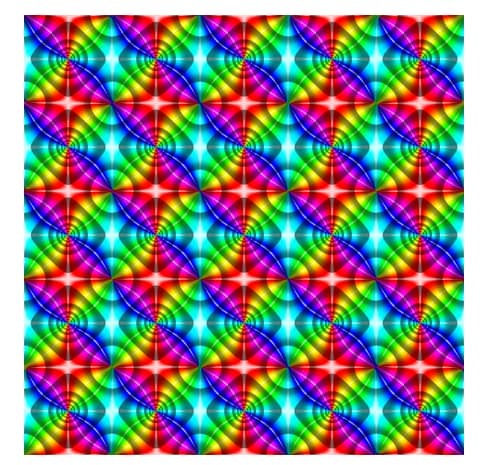
\includegraphics[width=\linewidth]{weierstrass_function.jpeg}
        \caption{Tracé de la fonction $\wp$ de Weierstrass par coloriage de domaine.}
    \end{figure}
    
    \newpage
    \begin{proposition}
    La fonction \( \wp \) est méromorphe dans \( \mathbb{C} \). Plus particulièrement :
    \begin{enumerate}
        \item \( \wp' \in \mathcal{H}\left( \mathbb{C}/\Lambda \right)\) et \( \wp'(z) = -2 \sum_{\gamma \in \Lambda} \frac{1}{(z - \gamma)^3} \)
        \item Tous les points du réseau \( \Lambda \) sont des pôles doubles de \( \wp \) de résidu 0
    \end{enumerate}
    \end{proposition}
    
    Pour montrer cette proposition ainsi que la bonne définition de \(\wp\), nous allons d'abord démontrer deux lemmes :
    
    \begin{lemma}
    Pour tout \(k \in \mathbb{N}^*\):
    \[
    \sum_{(n,m) \in T_k} \frac{1}{|\sigma_{n,m}|^3} \leq \frac{8}{\delta^3 k^2}
    \]
    où \(\delta = \min \{|\sigma_{n,m}|, (n,m) \in T_1\}\).
    \end{lemma}
    
    \begin{proof}[\textbf{Démonstration}]
    On a pour tout \(k > 0\):
    \[
    |T_k| = |\{(n,m) \in \mathbb{Z}^2, \max(|n|,|m|) \leq k\}| - |\{(n,m) \in \mathbb{Z}^2, \max(|n|,|m|) \leq k-1\}| = (2k+1)^2 - (2k-1)^2 = 8k
    \]
    \(T_k\) contient donc \(8k\) points.
    
    Ensuite, pour tout \((n,m) \in T_k\): \(|\sigma_{n,m}| \geq k\delta\). En effet, supposons sans perte de généralité \(|\tau_1| \geq |\tau_2|\) \\
    Nécessairement, \(\delta = |\tau_2| = |\sigma_{0,1}|\). Ainsi on a :
    \[
    |n\tau_1 + m\tau_2| \geq \max(|n|,|m|)|\tau_2| = k\delta
    \]
    On a alors immédiatement :
    \[
    \sum_{(n,m) \in T_k} \frac{1}{|\sigma_{n,m}|^3} \leq \sum_{(n,m) \in T_k} \frac{1}{(k\delta)^3} \leq \frac{8}{\delta^3 k^2}
    \]
    \end{proof}
    \begin{lemma}
        Pour tout \(\omega \in \Lambda\), la suite \((\Psi_{\omega, p})\) définie par
        \[
        \Psi_{\omega, p}(z) =  \sum_{k=1}^p \left( \sum_{(n,m) \in T_k, \sigma_{n,m} \neq \omega} \left( \frac{1}{(z - \sigma_{n,m})^2} - \frac{1}{\sigma_{n,m}^2} \right) \right)
        \]
        est uniformément convergente sur tout compact \(K \subset \mathbb{C} \setminus (\Lambda^{*} \setminus \omega)\).
        \end{lemma}
        
        \begin{proof}[\textbf{Démonstration}]
        \(K\) étant un compact, il existe un nombre \(r > 0\) tel que \(K \subset B(0,r)\). Ainsi, puisque pour tout \(z \in K\) et tout \(|\sigma_{n,m}| = |n \tau_1 + m \tau_2| > 2r\) :
        \[
        \left| \frac{1}{(z - \sigma_{n,m})^2} - \frac{1}{\sigma_{n,m}^2} \right| = \left| \frac{\sigma_{n,m}^2 - (z^2 - 2z\sigma_{n,m} + \sigma_{n,m}^2)}{\sigma_{n,m}^2 (z - \sigma_{n,m})^2} \right|
        \]
        \[
        = \left| \frac{z(z - 2\sigma_{n,m})}{\sigma_{n,m}^2 (z - \sigma_{n,m})^2} \right|
        \]
        \[
        = \frac{|z| \left| 2 - \frac{z}{\sigma_{n,m}} \right|}{|\sigma_{n,m}|^3 \left| 1 - \frac{z}{\sigma_{n,m}} \right|^2} 
        \]
        \[
        < \frac{10r}{|\sigma_{n,m}|^3}
        \]
        
        On obtient ainsi, d'après le lemme précédent, que pour tout couple d'entier \( j > l > \frac{2r}{\delta} \):
        \[
        \sup_{z \in K} | \Psi_{w,j}(z) - \Psi_{w,l}(z) | \leq \sup_{z \in K} \left| \sum_{k=l+1}^{j} \sum_{(n,m) \in T_k, \sigma_{n,m} \neq \omega} \left( \frac{1}{(z - \sigma_{n,m})^2} - \frac{1}{\sigma_{n,m}^2} \right) \right|
        \]
        \[
        \leq 10r \sum_{k=l+1}^{j} \sum_{(n,m) \in T_k} \frac{1}{|\sigma_{n,m}|^3}
        \]
        \[
        \leq \frac{80r}{\delta^3} \sum_{k=l+1}^{j} \frac{1}{k^2}
        \]
        Par conséquent, \((\Psi_{w,p})_{p \in \mathbb{N}}\) est une suite de Cauchy sur \(K\) pour \(||\cdot||_{\infty}\), elle est donc uniformément convergente sur \(K\).
        \end{proof}
        
        Nous pouvons désormais démontrer la proposition 7.
        
        
        \begin{proof}[\textbf{Démonstration}] 
            \ 1. Pour montrer que la fonction \(\wp\) est bien définie sur \(\mathbb{C}/\Lambda\), on écrit :
        
        \[
        \wp(z) = \frac{1}{z^2} + \sum_{\gamma \in \Lambda^*} \left( \frac{1}{(z - \gamma)^2} - \frac{1}{\gamma^2} \right)
        \]
        \[
        = \frac{1}{z^2} + \sum_{k =1}^{ + \infty} \left( \sum_{(n,m) \in T_k} \left( \frac{1}{(z - \sigma_{n,m})^2} - \frac{1}{\sigma_{n,m}^2} \right) \right)
        \]
        \[
        = \frac{1}{z^2} + \lim_{p \to + \infty} \Psi_{0,p}(z)
        \]
        
        Ensuite, d'après le théorème de Weierstrass et le lemme 7, la fonction
        \[
        \Psi_{0}(z) = \lim_{p \to \infty} \Psi_{0,p}(z)
        \]
        est holomorphe dans \(\mathbb{C}/\Lambda^*\) et
        \[
        \Psi'_{0}(z) = \lim_{p \to \infty} \sum_{k=1}^{p} \left( \sum_{(n,m) \in T_k} \left( \frac{1}{(z - \sigma_{n,m})^2} - \frac{1}{\sigma_{n,m}^2} \right)' \right)
        \]
        \[
        = \sum_{k=1}^{ + \infty} \left( \sum_{(n,m) \in T_k} \left( -\frac{2}{(z - \sigma_{n,m})^3} \right) \right)
        \]
        \[
        = -2 \sum_{\gamma \in \Lambda^*} \frac{1}{(z - \gamma)^3}
        \]
        
        D'où
        \[
        \wp \in \mathcal{H}( \mathbb{C}/\Lambda) \quad \text{et} \quad \wp'(z) = -\frac{2}{(z)^3} + \Psi_0'(z) = -2 \sum_{\gamma \in \Lambda} \frac{1}{(z - \gamma)^3}
        \]
        
        2. D'après ce qui précède :
        
        \[
        \wp(z) = \frac{1}{z^2} + \Psi_0(z)
        \]
        
        avec \(\Psi_0\) une fonction holomorphe sur \(\mathbb{C} \setminus \Lambda^*\), donc au voisinage de 0. Ainsi, la fonction \(\wp\) possède en 0 un pôle double de résidu 0.
        
        Maintenant, soit \(\omega \in \Lambda^*\), posons
        
        \[
        \Psi_\omega(z) = \lim_{p \to +\infty} \Psi_{\omega, p}(z) = \sum_{\gamma \in \Lambda^* \setminus \{\omega\}} \left( \frac{1}{(z - \gamma)^2} - \frac{1}{\gamma^2} \right)
        \]
        
        Alors, puisque \(\Psi_\omega \in \mathcal{H}(\mathbb{C} \setminus (\Lambda^* \setminus \{\omega\}))\) et
        
        \[
        \wp(z) = \frac{1}{z^2} + \Psi_\omega(z) + \left( \frac{1}{(z - \omega)^2} - \frac{1}{\omega^2} \right)
        \]
        
        la fonction \(\wp\) possède en \(\omega\) un pôle double de résidu 0.
        \end{proof}
        \begin{remark}
            Le réseau \(\Lambda\) étant symétrique par rapport à l'origine, on a :
            \[
            \sum_{\gamma \in \Lambda^*} \left( \frac{1}{(z - \gamma)^2} - \frac{1}{\gamma^2} \right) = \sum_{\gamma \in \Lambda^*} \left( \frac{1}{(z + \gamma)^2} - \frac{1}{\gamma^2} \right)
            \]
            \end{remark}
            
            \subsubsection{Propriétés de la fonction \(\wp\)}
            
            \begin{proposition}
            La fonction \(\wp\) est paire.
            \end{proposition}
            
            \begin{proof}[\textbf{Démonstration}] 
            Pour tout \(z \in \mathbb{C} \setminus \Lambda\) :
            \[
            \wp_\Lambda(-z) = \frac{1}{z^2} + \sum_{\gamma \in \Lambda^*} \left( \frac{1}{(-z - \gamma)^2} - \frac{1}{\gamma^2} \right)
            = \frac{1}{z^2} + \sum_{\gamma \in \Lambda^*} \left( \frac{1}{(z + \gamma)^2} - \frac{1}{\gamma^2} \right)
            = \wp_\Lambda(z)
            \]
            \end{proof}
            
            \begin{proposition}
            \((\tau_1, \tau_2)\) est une paire de périodes fondamentales de la fonction \(\wp\). Autrement dit, \(\Lambda_{\wp} = \Lambda^*\).
            \end{proposition}
            
            \begin{proof}[\textbf{Démonstration}] 
            Il n'est pas évident de voir que \(\tau_1\) et \(\tau_2\) soient deux périodes de la fonction \(\wp\). En revanche, pour la fonction \(\wp'\) c'est clair. En effet, remplacer \(z\) par \(z + \tau_i\) (\(i = 1, 2\)) dans l'expression de \(\wp'\) revient à effectuer une bijection sur les indices, qui laisse invariante la somme.
            
            On a donc pour tout \(z \in \mathbb{C} \setminus \Lambda\) :
            \[
            \wp'(z + \tau_j) - \wp'(z) = 0 \quad j = 1, 2
            \]
            
            Ainsi, \(\mathbb{C} \setminus \Lambda\) étant un domaine (ouvert connexe de \(\mathbb{C}\)), il existe deux constantes \(c_1\) et \(c_2\) telles que pour tout \(z \in \mathbb{C} \setminus \Lambda\) :
            \[
            \wp(z + \tau_j) - \wp(z) = c_j \quad j = 1, 2
            \]
            
            Ainsi, en prenant \(z = -\frac{\tau_j}{2}\), on a, \(\wp\) étant une fonction paire, que :
            \[
            c_j = \wp\left(\frac{\tau_j}{2}\right) - \wp\left(-\frac{\tau_j}{2}\right) = 0
            \]
            
            Par conséquent, \(\tau_1\) et \(\tau_2\) sont deux périodes de la fonction \(\wp\). D'où \(\Lambda^* \subset \Lambda_{\wp}\).
            
            Montrons à présent l'inclusion réciproque. Pour cela, soit \(\tau \in \Lambda_{\wp}\). Alors, puisque l'origine est un pôle double de la fonction \(\wp\) d'après la proposition 7, on a :
            \[
            \lim_{h \to 0} h^2 \wp(\tau + h) = \lim_{h \to 0} h^2 \wp(h) = l \neq 0
            \]
            
            Par conséquent, la fonction \(\wp\) possédant un pôle double en \(\tau\), on a que \(\tau \in \Lambda^*\).
            \end{proof}
            
            \begin{theorem}
            La fonction \(\wp\) est elliptique paire d'ordre 2 qui admet \((\tau_1, \tau_2)\) pour périodes fondamentales.
            \end{theorem}
            
            \begin{proposition}
            \(\wp'\) est une fonction elliptique impaire d'ordre 3 dont \((\tau_1, \tau_2)\) est une paire de périodes fondamentales. De plus, dans \(P_{\wp'} (\tau_1, \tau_2)\) :
            \begin{enumerate}
                \item 0 est son unique pôle. C'est un pôle triple de résidu 0.
                \item \(\frac{\tau_1}{2}\), \(\frac{\tau_2}{2}\), et \(\frac{\tau_1 + \tau_2}{2}\) sont ses trois uniques zéros (simples).
            \end{enumerate}
            \end{proposition}
            
            \begin{proof}[\textbf{Démonstration}] 
            1. Nous avons déjà vu dans la précédente démonstration que la fonction \(\wp'\) est périodique avec pour périodes fondamentales le couple \((\tau_1, \tau_2)\).
            
            Ensuite, on a :
            \[
            \wp'(z) = \frac{-2}{z^3} + \Psi_0'(z)
            \]
            et \(\Psi_0' \in \mathcal{H}(\mathbb{C} \setminus \Lambda^*)\), son unique pôle dans \(P_{\wp'} (\tau_1, \tau_2)\) est un pôle triple en 0 de résidu 0.
            
            Ainsi, la fonction dérivée \(\wp'\) est une fonction elliptique impaire (car \(\wp\) est paire) d'ordre 3 dont \((\tau_1, \tau_2)\) est une paire de périodes fondamentales.
            
            2. Soit \(z_0 \in \left\{ \frac{\tau_1}{2}, \frac{\tau_2}{2}, \frac{\tau_1 + \tau_2}{2} \right\}\). Alors,
            \[
            \wp'(z_0) = -\wp'(-z_0) = \wp'(-z_0 + 2z_0) = -\wp'(z_0) \implies \wp'(z_0) = 0
            \]
            
            Ainsi, \(\frac{\tau_1}{2}\), \(\frac{\tau_2}{2}\), et \(\frac{\tau_1 + \tau_2}{2}\) sont les trois uniques zéros (simples) de la fonction \(\wp'\) dans \(P_{\wp'} (\tau_1, \tau_2)\).
            \end{proof}
            \begin{definition}
                On définit pour tout \(j \in \mathbb{N}, j \geq 3\) :
                \[
                G_j(\Lambda) = \sum_{\gamma \in \Lambda^*} \frac{1}{\lambda^j}
                \]
                \end{definition}
                
                Passons maintenant à un lemme important concernant la sommabilité d'une certaine famille de termes.
                
                \begin{lemma}
                La famille \(\left( \frac{1}{|\gamma|^\alpha} \right)_{\gamma \in \Lambda^*}\) est sommable pour \(\alpha > 2\).
                \end{lemma}
                
                \begin{proof}[\textbf{Démonstration}] 
                Nous avons déjà démontré le cas \(\alpha = 3\) plus haut, mais nous aurons besoin du cas général pour la suite.
                
                \[
                \sum_{\gamma \in \Lambda^*} \frac{1}{|\gamma|^\alpha} = \sum_{k=1}^{+\infty} \left( \sum_{(n,m) \in T_k} \frac{1}{|\sigma_{n,m}|^\alpha} \right)
                \]
                
                \[
                \leq \sum_{k=1}^{+\infty} \left( \sum_{(n,m) \in T_k} \frac{1}{(k\delta)^\alpha} \right)
                \]
                
                \[
                \leq \sum_{k=1}^{+\infty} \left( \frac{8k}{(k\delta)^\alpha} \right)
                \]
                
                \[
                = \frac{8}{\delta^\alpha} \sum_{k=1}^{+\infty} \frac{1}{k^{\alpha-1}}
                \]
                
                Cette série est convergente car \(\alpha > 2\).
                \end{proof}
                
                \section*{Développement de Laurent au Voisinage de Zéro}
                
                Cherchons à présent le développement de Laurent de \(\wp\) au voisinage de zéro. Pour ce faire, posons la fonction \(f\) définie par 
                
                \[
                f(z) = \sum_{\gamma \in \Lambda^*} \left( \frac{1}{(z+\gamma)^2} - \frac{1}{\gamma^2} \right),
                \]
                
                qui est holomorphe au voisinage de 0 d'après les différents lemmes qui précèdent. De plus, les dérivées successives de \(f\) se calculent aisément en dérivant terme à terme sous le signe \(\sum\) :
                
                \[
                f^{(n)}(z) = (-1)^n (n+1)! \sum_{\gamma \in \Lambda^*} \frac{1}{(z+\gamma)^{n+2}}
                \]
                
                En prenant \(z=0\), il vient
                
                \[
                f^{(n)}(0) = (-1)^n (n+1)! \sum_{\gamma \in \Lambda^*} \frac{1}{\gamma^{n+2}}
                \]
                
                On rappelle de plus que si \(\gamma \in \Lambda^*\), on a aussi \(-\gamma \in \Lambda^*\). La famille \(\left(\frac{1}{\gamma^{n+2}} \right)_{\gamma \in \Lambda^*}\) étant sommable, nous pouvons réorganiser l'ordre des termes dans le calcul de la somme. Ainsi, si \(n\) est impair, la somme
                \[
                \frac{1}{\gamma^{n+2}} + \frac{1}{(-\gamma)^{n+2}}
                \]
                est nulle, donc aussi \(f^{(n)}(0)\). Finalement, la formule de Taylor nous donne le développement en série entière de \(f\) à l'origine, donc le développement de Laurent de \(\wp\) :
                
                Au voisinage de 0 on a :
                
                \[
                \wp(z) = \frac{1}{z^2} + f(z)
                \]
                
                \[
                = \frac{1}{z^2} + \sum_{n=1}^{+\infty} \left( \frac{(-1)^n (n+1)!}{n!} \sum_{\gamma \in \Lambda^*} \frac{1}{\gamma^{n+2}} \right) z^n
                \]
                
                \[
                = \frac{1}{z^2} + \sum_{n=1}^{+\infty} \left( \sum_{\gamma \in \Lambda^*} \frac{2n+1}{\gamma^{2n+2}} \right) z^{2n}
                \]
                
                \[
                = \frac{1}{z^2} + \sum_{n=1}^{+\infty} \left( (2n+1) G_{2n+2} \right) z^{2n}
                \]
                
                \section*{Équation Différentielle}
                
                Nous allons maintenant démontrer que la fonction \(\wp\) est solution d'une équation différentielle particulière.
                
                \begin{theorem}
                La fonction \(\wp\) est solution de l'équation différentielle :
                \[
                \ u'^2 = 4u^3 - 60G_4 u - 140G_6
                \]
                \end{theorem}
                
                \begin{proof}[\textbf{Démonstration}] 
                On a les développements limités au voisinage de 0 suivants :
                
                \[
                \wp(z) = \frac{1}{z^2} + 3G_4z^2 + 5G_6z^4 + O(z^5)
                \]
                
                \[
                \wp'(z) = \frac{-2}{z^3} + 6G_4z + 20G_6z^3 + O(z^4)
                \]
                
                \[
                \wp'(z)^2 = \frac{4}{z^6} -  \frac{24G_4}{z^2} + 80G_6 + O(z)
                \]
                
                \[
                \wp(z)^3 = \frac{1}{z^6} + \frac{9G_4}{z^2}+ 15G_6 + O(z)
                \]
                
                Ainsi, un simple calcul montre que l'on a :
                
                \[
                \wp'^2(z) - 4\wp^3(z) + 60G_4\wp(z) + 140G_6 = O(z)
                \]
                
                Par conséquent, la fonction \(\wp'^2 - 4\wp^3 + 60G_4\wp + 140G_6\) est une fonction entière elliptique. Ainsi, par le Théorème 1, elle est constante. Cette constante étant nulle (il suffit de prendre la limite \(z \to 0\)), on obtient alors :
                
                \[
                \wp'^2 = 4\wp^3 - 60G_4\wp - 140G_6
                \]
                \end{proof}
                
                Dans la suite, on pose :
                
                \[
                g_2 = g_2(\Lambda) = 60G_4
                \]
                \[
                g_3 = g_3(\Lambda) = 140G_4
                \]
                
                L'équation différentielle s'écrit alors :
                
                \[
                u'^2 = 4u^3 - g_2u - g_3
                \]
                
                \begin{corollary}
                    Le polynôme \(f = 4X^3 - g_2X - g_3\) possède trois zéros distincts, à savoir \(\wp\left(\frac{\tau_1}{2}\right)\), \(\wp\left(\frac{\tau_2}{2}\right)\) et \(\wp\left(\frac{\tau_1 + \tau_2}{2}\right)\) et par conséquent on a, pour tout réseau \(\Lambda\), \(g_2(\Lambda)^3 - 27g_3(\Lambda)^2 \neq 0\).
                    \end{corollary}
                    
                    \begin{proof}[\textbf{Démonstration}] 
                    La première partie provient du fait que \(f(\wp) = \wp'^2\) et que les trois uniques zéros de \(\wp'\) dans \(P(\tau_1, \tau_2)\) sont 
                    \(\frac{\tau_1}{2}\), \(\frac{\tau_2}{2}\), et \(\frac{\tau_1 + \tau_2}{2}\). De plus, les trois valeurs \(\wp\left(\frac{\tau_1}{2}\right)\), \(\wp\left(\frac{\tau_2}{2}\right)\) et \(\wp\left(\frac{\tau_1 + \tau_2}{2}\right)\)
                    sont distinctes deux à deux, sinon pour \(j = 1, 2\) l'équation \(\wp(z) = \wp(\frac{\tau_j}{2})\) aurait quatre solutions dans \(P(\tau_1, \tau_2)\) au lieu de 2,
                    qui est l'ordre de la fonction \(\wp\), ce qui est en contradiction avec le corollaire 1.
                    
                    Enfin, on sait que l'équation \(x^3 + px + q = 0\) possède une racine double si et seulement si \(\Delta = 4p^3 + 27q^2 = 0\).
                    
                    Ainsi, en considérant l'équation \(4x^3 - g_2(\Lambda)x - g_3(\Lambda) = 0\), dont nous venons de trouver les 3 solutions distinctes deux à deux, on a :
                    
                    \[
                    4\left(-\frac{g_2(\Lambda)}{4}\right)^3 + 27\left(-\frac{g_3(\Lambda)}{4}\right)^2 \neq 0 \implies g_2(\Lambda)^3 - 27g_3(\Lambda)^2 \neq 0
                    \]
                    \end{proof}
                    \subsubsection{Application aux fonctions elliptiques.}
                    \begin{lemma}
                    Soit \(z_0 \in P(\tau_1, \tau_2)\). Alors :
                    \begin{enumerate}
                        \item Si \(z_0 \notin \left\{ 0, \frac{\tau_1}{2}, \frac{\tau_2}{2}, \frac{\tau_1 + \tau_2}{2} \right\}\), \(z_0\) est un zéro simple de la fonction \(\wp - \wp(z_0)\).
                        \item Si \(z_0 \in \left\{ \frac{\tau_1}{2}, \frac{\tau_2}{2}, \frac{\tau_1 + \tau_2}{2} \right\}\), \(z_0\) est un zéro double de la fonction \(\wp - \wp(z_0)\).
                    \end{enumerate}
                    \end{lemma}
                    
                    \begin{proof}[\textbf{Démonstration}] 
                    1. Soit \(z_0 \notin \left\{ 0, \frac{\tau_1}{2}, \frac{\tau_2}{2}, \frac{\tau_1 + \tau_2}{2} \right\}\). Alors \(\zeta_{- z_0} \neq z_0\), où \(\zeta_{- z_0}\) est l'unique point de \(P(\tau_1, \tau_2)\) tel que \(-z_0 = \zeta_{- z_0} + n\tau_1 + m\tau_2\).
                    
                    En effet, si $\zeta_{- z_0} = z_0$, on aurait
                    \[
                    z_0 = \frac{n\tau_1 + m\tau_2}{2}
                    \]                    
                    
                    En prenant \(n, m = - 1\) ou 0, nous aboutissons à une absurdité. Ainsi, la fonction \(\wp(z) - \wp(z_0)\) étant paire et elliptique d'ordre 2, \(z_0\) et $\zeta_{- z_0}$ sont ses deux uniques zéros dans \(P(\tau_1, \tau_2)\).
                    
                    2. Soit \(z_0 \in \left\{ \frac{\tau_1}{2}, \frac{\tau_2}{2}, \frac{\tau_1 + \tau_2}{2} \right\}\). Alors, \(z_0\) est un zéro simple de la fonction \(\wp'\), donc un zéro double de la fonction \(\wp - \wp(z_0)\).
                    \end{proof}
                    
                    \begin{lemma}
                    Si \(z_0 \in \left\{ 0, \frac{\tau_1}{2}, \frac{\tau_2}{2}, \frac{\tau_1 + \tau_2}{2} \right\}\) est un pôle ou un zéro d'une fonction elliptique paire \(f\) de périodes \(\tau_1\) et \(\tau_2\), il est d'ordre pair.
                    \end{lemma}
                    
                    \begin{proof}[\textbf{Démonstration}] 
                    Pour commencer, on va supposer que \(z_0\) est un zéro de \(f\). Alors on a (car \(f\) est paire) :
                    
                    \[
                    f^{(2n+1)}(z_0) = -f^{(2n+1)}(-z_0) = -f^{(2n+1)}(-z_0 + 2z_0) = -f^{(2n+1)}(z_0)
                    \]
                    
                    On a donc pour tout \(n \in \mathbb{N}\) :
                    
                    \[
                    f^{(2n+1)}(z_0) = 0
                    \]
                    
                    Par ailleurs, la fonction \(f\) étant elliptique (donc non constante) :
                    
                    \[
                    \exists m, R > 0, \forall z \in B(z_0, R) \quad f(z) = \sum_{n=m}^{+\infty} c_{2n} (z - z_0)^{2n} \quad c_{2m} \neq 0
                    \]
                    
                    Par conséquent, la fonction \(f\) admet un zéro d'ordre \(2m\) en \(z_0\).
                    
                    Supposons à présent que \(f\) possède un pôle d'ordre \(p\) en \(z_0\). Alors, la fonction \(\frac{1}{f}\) possède un zéro d'ordre \(p\) en \(z_0\) qui, d'après ce qui précède, est pair.
                    \end{proof}
                    
                    \begin{lemma}
                    Toute fonction elliptique \(f\) de période \(\tau_1\) et \(\tau_2\) possède au moins un zéro et un pôle dans \(P_{\wp}(\tau_1, \tau_2)\).
                    \end{lemma}
                    
                    \begin{proof}[\textbf{Démonstration}] 
                    La fonction \(f\) étant elliptique, son ordre \(m \geq 2\), possède donc au moins un zéro \(\zeta\) dans son parallélogramme fondamental \(P_f(\omega_1, \omega_2)\). Ainsi, puisqu'il existe \(n, m \in \mathbb{Z}, a \in P_{\wp}(\tau_1, \tau_2)\) tel que \(\zeta = a + n\tau_1 + m\tau_2\),
                    
                    On a, \(\tau_1\) et \(\tau_2\) étant deux périodes de \(f\), que 
                    
                    \[
                    0 = f(\zeta) = f(a + n\tau_1 + m\tau_2) = f(a)
                    \]
                    
                    De même, la fonction \(f\) possédant au moins un pôle \(\omega\) dans \(P_f(\omega_1, \omega_2)\), par conséquent, l'unique point \(b \in P_{\wp}(\tau_1, \tau_2)\) tel que
                    
                    \[
                        \omega = b + n\tau_1 + m\tau_2
                    \]
                    est un pôle de f (proposition 3).
                \end{proof}
                \begin{theorem}
                    Toute fonction elliptique \(f\) de périodes \(\tau_1\) et \(\tau_2\) est une fraction rationnelle de \(\wp\) et \(\wp'\).
                    \end{theorem}
                    
                    \begin{proof}[\textbf{Démonstration}]
                    Supposons pour commencer que \(f\) est paire et n'a ni zéro ni pôle en 0 et soit \(a \in P_{\wp}(\tau_1, \tau_2)\) un zéro de la fonction \(f\) (un tel \(a\) existe par ce qui précède). Alors, \(a \neq 0\) et pour l'unique point \(\zeta_{- a}\) de \(P_{\wp}(\tau_1, \tau_2)\) tel que :
                    
                    \[
                    -a = (\zeta_{- a} + n\tau_1 + m\tau_2)
                    \]
                    
                    on a alors :
                    
                    \begin{enumerate}
                        \item 
                        \[
                        \left\{
                        \begin{array}{ll}
                            a = \zeta_{-a} \text{ si } a \in \left\{\frac{\tau_1}{2}, \frac{\tau_2}{2}, \frac{\tau_1 + \tau_2}{2}\right\} \\ \\
                            a \neq \zeta_{-a} \text{ si } a \notin \left\{\frac{\tau_1}{2}, \frac{\tau_2}{2}, \frac{\tau_1 + \tau_2}{2}\right\}
                        \end{array}
                        \right.
                        \]
                        
                        \item 
                        \[
                        (c, d \in P_{\wp}(\tau_1, \tau_2) \text{ et } d \neq c, \zeta_{-c}) \implies \zeta_{-d} \neq c, \zeta_{-c}
                        \]
                        
                        \item Si \(a\) est un zéro d'ordre \(p\), alors \(\zeta_{-a}\) est aussi un zéro d'ordre \(p\) de \(f\). En effet, \(\zeta_{-a}\) et \(-a\) sont deux zéros de \(f\) de même multiplicité (proposition 3) ainsi que \(-a\) et \(a\) car :
                        \[
                        \lim_{h \to 0} \frac{f(-a + h)}{h^p} = (-1)^p \lim_{h \to 0} \frac{f(a + h)}{h^p}
                        \]
                    \end{enumerate}
                    
                    Par ailleurs, on désigne par \(a_1, \zeta_{-a_1}, \ldots, a_n, \zeta_{-a_n}\), la suite de tous les zéros de \(f\) dans \(P_{\wp}(\tau_1, \tau_2)\). Un zéro d'ordre \(p\) étant répété \(p\) fois s'il n'appartient pas à \(\left\{ \frac{\tau_1}{2}, \frac{\tau_2}{2}, \frac{\tau_1 + \tau_2}{2} \right\} \text{ et } \frac{p}{2}\) fois sinon (lemme 10).
                    
                    Ainsi la fonction 
                    
                    \[
                    (\wp - \wp(a_1)) \cdots (\wp - \wp(a_n))
                    \]
                    
                    a exactement les mêmes zéros (comptés avec multiplicité) que \(f\) dans \(P_{\wp}(\tau_1, \tau_2)\) (lemme 9) donc dans \(\mathbb{C}\) (proposition 3). De même, si \(b_1, \zeta_{-b_1}, \ldots, b_n, \zeta_{-b_n}\) sont les pôles de \(f\) dans \(P_{\wp}(\tau_1, \tau_2)\), la fonction 
                    
                    \[
                    \frac{1}{(\wp - \wp(b_1)) \cdots (\wp - \wp(b_n))}
                    \]
                    
                    a exactement les mêmes pôles, ainsi que leurs ordres respectifs, que \(f\) dans \(P_{\wp}(\tau_1, \tau_2)\) donc dans \(\mathbb{C}\) (proposition 3). Finalement, puisque \(n = m\) (Théorème 3),
                    
                    \[
                    \frac{(\wp - \wp(b_1)) \cdots (\wp - \wp(b_n))}{(\wp - \wp(a_1)) \cdots (\wp - \wp(a_n))} \cdot f
                    \]
                    
                    est une fonction entière périodique, elle est donc constante (Théorème 1).
                    
                    D'où
                    
                    \[
                    f = c \frac{(\wp - \wp(a_1)) \cdots (\wp - \wp(a_n))}{(\wp - \wp(b_1)) \cdots (\wp - \wp(b_n))} \quad \text{avec } c \in \mathbb{C}^*
                    \]
                    
                    À présent, supposons que la fonction paire \(f\) possède un zéro ou un pôle d'ordre \(2k\) en 0 (lemme 10). Alors, en posant :
                    
                    \[
                    j = \begin{cases} 
                        k & \text{si } 0 \text{ est un zéro de } f \\
                        -k & \text{si } 0 \text{ est un pôle de } f 
                        \end{cases}
                    \]
                    
                    la fonction \(\wp^j f\) devient une fonction elliptique de périodes \(\tau_1\) et \(\tau_2\) n’ayant ni zéro ni pôle en 0. On peut donc lui appliquer le résultat précédent.
                    
                    Pour finir, supposons que la fonction elliptique \(f\) n’est pas paire et posons
                    
                    \[
                    f_1(z) = \frac{f(z) + f(-z)}{2} \quad \text{et} \quad f_2(z) = \frac{f(z) - f(-z)}{2}
                    \]
                    
                    Alors, les deux fonctions \(f_1\) et \(\frac{f_2}{\wp'}\) sont paires de périodes \(\tau_1\) et \(\tau_2\). Ainsi, puisque
                    
                    \[
                    f = f_1 + \wp' \frac{f_2}{\wp'}
                    \]
                    
                    on obtient que la fonction \(f\) est une fonction rationnelle de \(\wp\) et \(\wp'\).
                    \end{proof}
                    \begin{theorem}
                        La fonction $\wp$ vérifie la relation algébrique suivante :
                        \[
                        (\wp')^2 = 4 \left( \wp - \wp\left( \frac{\tau_1}{2} \right) \right) \left( \wp - \wp\left( \frac{\tau_2}{2} \right) \right) \left( \wp - \wp\left( \frac{\tau_1 + \tau_2}{2} \right) \right)
                        \]
                        \end{theorem}
                        
                        \begin{proof}[\textbf{Démonstration}]
                        
                        Pour établir ce résultat, nous allons introduire une fonction auxiliaire et analyser ses propriétés. Commençons par définir la fonction suivante :
                        
                        \[
                        f = \left( \wp - \wp\left( \frac{\tau_1}{2} \right) \right) \left( \wp - \wp\left( \frac{\tau_2}{2} \right) \right) \left( \wp - \wp\left( \frac{\tau_1 + \tau_2}{2} \right) \right)
                        \]
                        
                        Ensuite, considérons le quotient suivant :
                        
                        \[
                        \frac{(\wp')^2}{f}
                        \]
                        
                        Selon la proposition 11 et le lemme 9, ce quotient est une fonction entière, doublement périodique. Par conséquent, d'après le Théorème 1, cette fonction est constante. Nous devons maintenant déterminer cette constante. Pour ce faire, examinons la limite suivante :
                        
                        \[
                        \psi_0(z) = \lim_{p \to +\infty} \psi_{0,p}(z) = \sum_{\gamma\in \Lambda ^* } \left( \frac{1}{(z - \gamma)^2} - \frac{1}{\gamma^2} \right)
                        \]
                        
                        Notons que $\psi_0$ appartient à $\mathcal{H}(\mathbb{C} \setminus \Lambda^*)$ et que dans $\mathbb{C}$, nous avons :
                        
                        \[
                        \wp(z) = \frac{1}{z^2} + \psi_0(z)
                        \]
                        
                        En effectuant un calcul simple, nous obtenons :
                        
                        \[
                        \lim_{z \to 0} \frac{(\wp')^2(z)}{f(z)} = 4
                        \]
                        
                        Nous pouvons donc conclure que la constante est égale à 4, ce qui achève la démonstration.
                        \end{proof}
                        \subsection{Fonction Zêta de Weierstrass}
                        \textit{Cette section est extraite de \url{https://mathworld.wolfram.com/WeierstrassZetaFunction.html}}
                        \subsubsection{Définition}
                        La fonction zêta de Weierstrass $\zeta (z; g_2, g_3)$ est la fonction quasipériodique définie par
                        \[
                        \frac{d \zeta (z; g_2, g_3)}{dz} \equiv -\wp (z; g_2, g_3), \tag{1}
                        \]
                        où $\wp (z; g_2, g_3)$ est la fonction elliptique de Weierstrass avec invariants $g_2$ et $g_3$, avec
                        \[
                        \lim_{z \to 0} \left[ \zeta (z; g_2, g_3) - z^{-1} \right] = 0. \tag{2}
                        \]
                        
                        Comme dans le cas des autres fonctions elliptiques de Weierstrass, les invariants elliptiques $g_2$ et $g_3$ sont fréquemment supprimés pour des raisons de compacité.
                        \begin{figure}
                            \centering
                            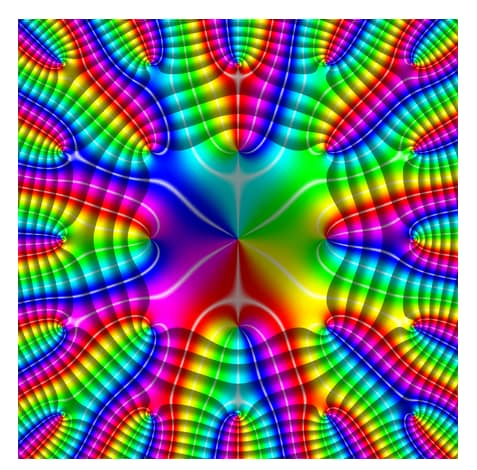
\includegraphics[width=\linewidth]{fonction_zeta.jpeg}
                            \caption{Tracé de la fonction zêta de Weierstrass par coloriage de domaine.}
                        \end{figure}

                        \newpage
                        \subsubsection{Remarque}
                        En utilisant la définition ci-dessus, on obtient
                        \[
                        \zeta (z) - z^{-1} = - \int_{0}^{z} \left[ \wp (z) - z^{-2} \right] dz \tag{3}
                        \]
                        \[
                        = - \sum_{m,n=-\infty}^{\infty} \int_{0}^{z} \left[ (z - \Omega_{mn})^{-2} - \Omega_{mn}^{-2} \right] dz, \tag{4}
                        \]
                        où $\Omega_{mn} = 2 m \omega_1 + 2 n \omega_2$, alors
                        \[
                        \zeta (z) = z^{-1} + \sum_{m,n=-\infty}^{\infty} \left[ (z - \Omega_{mn})^{-1} + \Omega_{mn}^{-1} + z \Omega_{mn}^{-2} \right] \tag{5}
                        \]
                        L'intégration $\wp (z + 2 \omega_1) = \wp (z)$ donne
                        \[
                        \zeta (z + 2 \omega_1) = \zeta (z) + 2 \eta_1. \tag{6}
                        \]
                        Laisser $z = -\omega_1$ donne
                        \[
                        \zeta (-\omega_1) + 2 \eta_1 = -\zeta (\omega_1) + 2 \eta_1, \tag{7}
                        \]
                        donc
                        \[
                        \eta_1 = \zeta (\omega_1). \tag{8}
                        \]
                        De la même manière,
                        \[
                        \eta_2 = \zeta (\omega_2). \tag{9}
                        \]
                        
                        D'après Whittaker et Watson (1990),
                        \[
                        \eta_1 \omega_2 - \eta_2 \omega_1 = \frac{1}{2} \pi i. \tag{10}
                        \]
                        
                        Si $x + y + z = 0$ donc
                        \[
                        \left[ \zeta (x) + \zeta (y) + \zeta (z) \right]^2 + \zeta' (x) + \zeta' (y) + \zeta' (z) = 0 \tag{11}
                        \]
                        
                        (Whittaker et Watson 1990, p. 446). Aussi,
                        \[
                            2 \frac{\begin{vmatrix}
                                1 & \wp (x) & \wp^2 (x) \\
                                1 & \wp (y) & \wp^2 (y) \\
                                1 & \wp (z) & \wp^2 (z)
                                \end{vmatrix}}{\begin{vmatrix}
                                    1 & \wp (x) & \wp' (x) \\
                                    1 & \wp (y) & \wp' (y) \\
                                    1 & \wp (z) & \wp' (z)
                                    \end{vmatrix} }               
                        = \zeta (x + y + z) - \zeta (x) - \zeta (y) - \zeta (z) \tag{12}
                        \]
                        
                        (Whittaker et Watson 1990, p. 446).
                        
                        Le développement en série de $\zeta (z)$ est donné par
                        \[
                        \zeta (z) = z^{-1} - \sum_{k=2}^{\infty} \frac{c_k z^{2k-1}}{2k-1}, \tag{13}
                        \]
                        où
                        \[
                        c_2 = \frac{g_2}{20} \tag{14}
                        \]
                        \[
                        c_3 = \frac{g_3}{28} \tag{15}
                        \]
                        
                        et
                        \[
                        c_k = \frac{3}{(2k + 1)(k - 3)} \sum_{m=2}^{k-2} c_m c_{k-m} \tag{16}
                        \]
                        pour $k \geq 4$ (Abramowitz et Stegun 1972, p. 635). Les premiers coefficients sont donc
                        \[
                        c_4 = \frac{1}{3} c_2^2 \tag{17}
                        \]
                        \[
                        c_5 = \frac{3}{11} c_2 c_3 \tag{18}
                        \]
                        \[
                        c_6 = \frac{1}{39} \left( 2 c_2^3 + 3 c_3^2 \right) \tag{19}
                        \]
                        \[
                        c_7 = \frac{2}{33} c_2^2 c_3 \tag{20}
                        \]
                        \[
                        c_8 = \frac{5}{7293} \left( 11 c_2^4 + 36 c_3^2 c_2 \right) \tag{21}
                        \]
                        \subsection{Fonction Sigma de Weierstrass}
                        \textit{Cette section est extraite de \url{https://mathworld.wolfram.com/WeierstrassSigmaFunction.html}}
                        \subsubsection{Définition}
                        Pour bien comprendre la fonction sigma de Weierstrass, il est essentiel de commencer par sa définition formelle. La fonction sigma de Weierstrass est définie comme la fonction quasipériodique suivante :
                        \[
                        \frac{d}{dz} \ln \sigma (z; g_2, g_3) = \zeta (z; g_2, g_3), \tag{1}
                        \]
                        où $\zeta (z; g_2, g_3)$ est la fonction zêta de Weierstrass, et elle satisfait également la condition :
                        \[
                        \lim_{z \to 0} \frac{\sigma (z)}{z} = 1. \tag{2}
                        \]
                        

                        
                        \begin{figure}
                            \centering
                            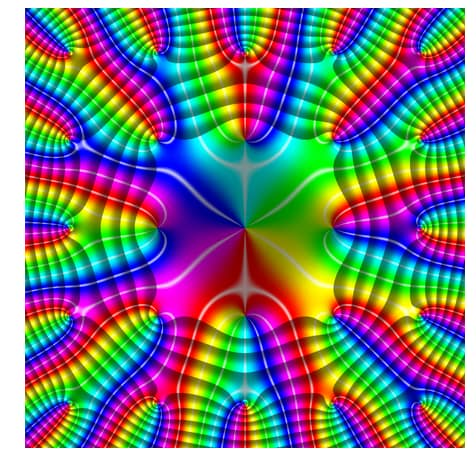
\includegraphics[width=\linewidth]{sigma_function.jpeg}
                            \caption{Tracé de la fonction sigma de Weierstrass par coloriage de domaine.}
                        \end{figure}
                        \newpage
                        Passons maintenant à quelques remarques importantes concernant cette fonction.
                        
                        \subsubsection{Remarque}
                        
                        
                        Comme dans le cas d'autres fonctions elliptiques de Weierstrass, les invariants $g_2$ et $g_3$ sont fréquemment supprimés par souci de compacité. Par conséquent, la fonction sigma peut être exprimée sous la forme :
                        \[
                        \sigma (z) = z \prod_{m,n=-\infty}^{\infty} \left( \left( 1 - \frac{z}{\Omega_{mn}} \right) \exp \left( \frac{z}{\Omega_{mn}} + \frac{z^2}{2 \Omega_{mn}^2} \right) \right), \tag{3}
                        \]
                        où le terme avec $m = n = 0$ est omis du produit et $\Omega_{mn} = 2 m \omega_1 + 2 n \omega_2$.
                        
                        
                        Il est également intéressant de noter une forme fermée spécifique de la fonction sigma. Étonnamment, $\sigma (1 | 1, i)/2$, où $\sigma (z | \omega_1, \omega_2)$ est la fonction sigma de Weierstrass avec des demi-périodes $\omega_1$ et $\omega_2$, a une forme fermée en termes de $\pi$, $e$, et $\Gamma \left( \frac{1}{4} \right)$. Cette constante est connue sous le nom de constante de Weierstrass.
                        
                        En outre, la fonction sigma satisfait aux relations de quasi-périodicité suivantes :
                        \[
                        \sigma (z + 2 \omega_1) = -e^{2 \eta_1 (z + \omega_1)} \sigma (z), \tag{4}
                        \]
                        \[
                        \sigma (z + 2 \omega_2) = -e^{2 \eta_2 (z + \omega_2)} \sigma (z), \tag{5}
                        \]
                        et
                        \[
                        \sigma_r (z) = \frac{e^{-\eta_r z} \sigma (z + \omega_r)}{\sigma (\omega_r)}, \tag{6}
                        \]
                        pour $r = 1, 2, 3$.
                        
                        Ces propriétés mettent en lumière la structure riche et complexe de la fonction sigma de Weierstrass. Elles jouent un rôle crucial dans de nombreuses applications théoriques et pratiques.
                                                

                        \subsection{Fonction êta de Weierstrass}
                        \textit{Cette section est extraite de Wikipedia.}

                        Pour mieux comprendre les fonctions elliptiques de Weierstrass, nous devons d'abord nous pencher sur la fonction êta de Weierstrass.
                        
                        \subsubsection{Définition}
                        
                        La fonction êta de Weierstrass est définie par
                        \[
                        \eta (w; \Lambda) = \zeta (z + w; \Lambda) - \zeta (z; \Lambda), \text{ pour tout } z \in \mathbb{C} \text{ et tout } w \text{ dans le réseau } \Lambda.
                        \]
                        
                        Cette fonction est bien définie, c'est-à-dire que
                        \[
                        \zeta (z + w; \Lambda) - \zeta (z; \Lambda) \text{ ne dépend que du vecteur } w.
                        \]
                        
                        \section{Domaine d'application des fonctions elliptiques de Weierstrass}
                        
                        Nous allons maintenant examiner les différentes applications des fonctions elliptiques de Weierstrass dans plusieurs domaines.
                        
                        \subsection*{1. Théorie des nombres et courbes elliptiques}
                        
                        Les fonctions elliptiques de Weierstrass jouent un rôle central dans la théorie des courbes elliptiques. Une courbe elliptique sur le plan complexe peut être paramétrée par la fonction $\wp(z)$ et sa dérivée $\wp'(z)$. Une courbe elliptique est définie par une équation de la forme :
                        
                        \[
                        y^2 = 4x^3 - g_2 x - g_3
                        \]
                        
                        \subsection*{2. Cryptographie}
                        
                        Les courbes elliptiques sont utilisées dans la cryptographie, notamment dans les algorithmes de cryptographie à clé publique comme l'ECC (Elliptic Curve Cryptography). Les propriétés algébriques des courbes elliptiques rendent ces algorithmes très efficaces et sûrs. Les fonctions de Weierstrass sont utilisées pour définir les courbes et les opérations arithmétiques sur les points de ces courbes.
                        
                        \subsection*{3. Théorie des fonctions spéciales}
                        
                        Les fonctions elliptiques sont des exemples fonctionnels de fonctions spéciales, qui apparaissent fréquemment dans divers domaines de l'analyse complexe et des équations différentielles. Par exemple, elles sont utilisées pour résoudre certaines équations différentielles non linéaires et pour l'étude des intégrales elliptiques.
                        
                        \subsection*{4. Mécanique et physique mathématique}
                        
                        En mécanique classique, les fonctions elliptiques apparaissent dans l'étude des mouvements périodiques et quasi-périodiques. Par exemple, elles sont utilisées pour résoudre le problème du pendule simple, où l'équation du mouvement peut être exprimée en termes de fonctions elliptiques.
                        
                        \subsection*{5. Géométrie algébrique}
                        
                        En géométrie algébrique, les courbes elliptiques sont des objets d'étude fondamentaux. Les fonctions de Weierstrass permettent de paramétrer ces courbes et de comprendre leurs propriétés géométriques et topologiques. Elles jouent un rôle clé dans des théorèmes importants, comme le théorème de Mordell-Weil, qui décrit la structure des points rationnels sur une courbe elliptique.
                        
                        \subsection*{6. Théorie des partitions de Rogers-Ramanujan}
                        
                        Les fonctions elliptiques apparaissent également dans la théorie des partitions, en particulier dans les identités de Rogers-Ramanujan, qui sont des résultats importants en combinatoire et en théorie des nombres. Ces identités peuvent être prouvées en utilisant des propriétés des fonctions elliptiques et des séries infinies.
                        
                        \subsection*{7. Intégration et fonctions transcendantes}
                        
                        Les intégrales de certaines fonctions rationnelles peuvent être exprimées en termes de fonctions elliptiques. Par exemple, les intégrales elliptiques sont liées aux fonctions de Weierstrass et permettent de résoudre des problèmes d'intégration complexes.

                        

                        \newpage
                        \section*{Conclusion}

            Au terme de cette exploration détaillée des fonctions elliptiques de Weierstrass, nous avons pu apprécier la profondeur et la beauté de ces
            fonctions dans le cadre de l'analyse complexe. Les propriétés uniques des fonctions $\wp$, zêta, êta et sigma de Weierstrass, couplées à leur élégante
            structure périodique et leurs implications en théorie des nombres et en cryptographie, illustrent parfaitement l'interconnexion entre la théorie 
            mathématique pure et ses applications pratiques. Ce voyage à travers les rappels fondamentaux et les aspects avancés des fonctions elliptiques a 
            non seulement renforcé notre compréhension de ces fonctions, mais a également ouvert des perspectives sur leur potentiel d'application dans des
            domaines aussi divers que la physique théorique et l'ingénierie. Enfin, l'étude des fonctions de Weierstrass souligne l'importance continue de
            l'analyse complexe dans le progrès scientifique et technologique.
            \newpage
            \section*{Bibliographie}
            
            \begin{thebibliography}{9}
            	
            	\bibitem{atindogbe2022}
            	Cyriaque Atindogbe, \textit{Documents de cours Analyse Complexe}, Mars 2022.
            	
            	\bibitem{wikipedia}
            	Wikipedia, \url{https://fr.m.wikipedia.org/wiki/Fonction_z%C3%AAta_de_Weierstrass}.
            	
            	\bibitem{wolfram1}
            	Wolfram MathWorld, \url{https://mathworld.wolfram.com/WeierstrassZetaFunction.html}.
            	
            	\bibitem{wolfram2}
            	Wolfram MathWorld, \url{https://mathworld.wolfram.com/WeierstrassSigmaFunction.html}.
            	
            	\bibitem{argoud}
            	Thomas Argoud, \textit{Travail d'étude de recherche sur les fonctions élliptiques}.
            	
            \end{thebibliography}

\end{document}